\chapter{Performance Evaluation of S-ALOHA in context of single Base Station}
\label{chapter:icc17}
% **************************** Define Graphics Path **************************
\ifpdf
    \graphicspath{{Chapter4/Figs/Raster/}{Chapter4/Figs/PDF/}{Chapter4/Figs/}}
\else
    \graphicspath{{Chapter4/Figs/Vector/}{Chapter4/Figs/}}
\fi
\qs{Based on ICC2017}
The S-ALOHA (i.e. slotted-ALOHA) protocol is recently regaining interest in Low Power Wide Area Networks (LPWAN) handling M2M traffic. Despite intensive studies since the birth of S-ALOHA, the special features of M2M traffic and requirements highlight the importance of analytical models taking into account performance-affecting factors and giving a thorough performance evaluation. In this chapter, we propose a low-complexity but still accurate analytical model capable of evaluating S-ALOHA in terms of packet loss rate, throughput, energy-efficiency and average number of transmissions. The proposed model is able to facilitate dimensioning and design of S-ALOHA based LPWAN. 

This chapter is organized as follows: Sec.~\ref{sec:icc17-introduction} is the introduction part. Sec.~\ref{sec:icc17-system-model} presents the system model. Sec.~\ref{sec:ideal_power_control} is the performance analysis about S-ALOHA in ideal systems, i.e., without power control and fading. Sec.~\ref{sec:imperfect-power-control} takes into account imperfect power control under wide-band system. Sec.~\ref{sec:simulation_result} proves the accuracy of proposed model by simulation and gives some deduced design guidelines. Sec.~\ref{sec:icc17-conclusion}concludes this chapter.

\section{Introduction}
\label{sec:icc17-introduction}
Machine-Type Communication (MTC) is expected to gain more popularity in the next decade. Low Power Wide Area Network (LPWAN) networks are regarded to be an attractive option for MTC~\cite{goursaud2015dedicated}. Due to its simplicity, the S-ALOHA (i.e. slotted-ALOHA) protocol is recently regaining interest in Low Power Wide Area Networks (LPWAN) handling M2M traffic. 

Despite intensive studies since the birth of S-ALOHA~\cite{abramson1970aloha}, the objectives of the existing related studies are usually analyzing throughput, packet loss rate, etc. In a radio communication system, factors such as capture effect, diversity of transmit power levels, power control precision, among with others, have a significant impact on ALOHA-like multiple access protocol. 

The special features of M2M traffic and requirements highlight the importance of analytical models taking into account performance-affecting factors and giving a thorough performance evaluation.
Fulfilling this necessity is the main focus of this chapter: we jointly consider the impact of capture effect, diversity of transmit power levels with imperfect power control. We propose a low-complexity but still accurate analytical model capable of evaluating S-ALOHA in terms of packet loss rate, throughput, energy-efficiency and average number of transmissions. The proposed model is able to facilitate dimensioning and design of S-ALOHA based LPWAN. The comparison between simulation and analytical results confirms the accuracy of our proposed model. The design guides about S-ALOHA based LPWAN deduced from our model are: the imperfect power control can be positive with capture effect and appropriate transmit power diversity strategy. The transmit power diversity strategy should be determined by jointly considering network charges level, power control precision and SINR threshold to achieve optimal performance of S-ALOHA.
 %~\cite{krishna1994comparison}.  

The rest of this chapter is organized as follows: Sec.~\ref{sec:icc17-system-model} presents the system model. Sec.~\ref{sec:ideal_power_control} is the performance analysis about S-ALOHA in ideal systems, i.e., without power control and fading. Sec.~\ref{sec:imperfect-power-control} takes into account imperfect power control under wide-band system. Sec.~\ref{sec:simulation_result} proves the accuracy of proposed model by simulation and gives some deduced design guidelines. Sec.~\ref{sec:icc17-conclusion}concludes this chapter.




\section{Related work}
Lots of researches related to ALOHA-like protocol have been done by taking into account some of the aforementioned factors. Lamaire et al.~\cite{lamaire1998randomization} derive the optimal transmit power distribution under three models: perfect capture model, signal-to-interference threshold with and without Rayleigh fading model. Altman et al.~\cite{altman2005slotted} propose to differentiate transmission priority by using different transmit power levels and convert it as a game problem. Both~\cite{lamaire1998randomization}\cite{altman2005slotted} ignore the impact of power control error for the transmit power distribution. 
Yang et al.~\cite{yang2012performance} analyze backoff algorithms for LTE Random Access Channel (RACH), which employ ALOHA-like protocol. Nielsen et al.~\cite{nielsen2015tractable} analyze the outage probability for LTE four-steps random access mechanism. Both~\cite{yang2012performance}\cite{nielsen2015tractable} use an analytical model adapted from Bianchi model~\cite{bianchi2000performance}. 
Zozor et al.~\cite{zozor2016time} study collision probability for the pure time-frequency ALOHA access via stochastic geometry approach and calculate the load capacity according to a maximal packet loss rate. 
Goursaud et al.~\cite{goursaud2016random} consider the carrier frequency uncertainty issue and study ALOHA protocol behavior. However \cite{yang2012performance}\cite{nielsen2015tractable}\cite{bianchi2000performance}\cite{zozor2016time}\cite{goursaud2016random} have not taken into account the capture effect and diversity of transmit power.
Bayrakdar et al.~\cite{bayrakdar2016slotted} evaluate the throughput performance of S-ALOHA based cognitive radio network under Rayleigh fading channels with capture effect, but with identical transmit power in each transmission. 


%The slotted ALOHA protocol~\cite{abramson1970aloha} has been studied at length since its born.
As far as we know, few works about S-ALOHA protocol jointly consider the impact of capture effect, power control error, diversity of transmit power levels, and give a multi-criteria performance analysis for M2M environment. In this chapter, we propose an analytical model to study the steady-state performance of S-ALOHA including packet loss rate, throughput, energy-efficiency and average number of transmission under the following situations: 
\begin{itemize}
	\item ideal system with perfect power control;
	\item wide-band system with imperfect power control,
	\item system with fading and imperfect power control.
\end{itemize} 
In the proposed model, the basic idea is to numerically obtain cumulative distribution function (CDF) of the total interference from its characteristic function (CF). This allows calculating the capture probability and thus the transmission failure probability for a single trial. We then use a fixed point analysis to calculate the steady state packet loss rate, throughput, energy-efficiency and average number of transmissions.
\section{System model}
\label{sec:icc17-system-model}
We consider a single base station. 
Terminals served by this base station employ S-ALOHA protocol to transmit packets. 
The behavior of different terminals is independent.
The time axis is divided into slots of fixed length $T$ equal to the transmission time of a single packet. 
The arrival of fresh packet is modeled as a stationary Poisson process with mean intensity $\lambda$. 
Thus, the average arrival rate of fresh packet in unit slot is $\alpha = \lambda T$. 

In terms of capture effect, Signal-to-Interference-and-Noise ratio (SINR) threshold model is applied. 
In such a model, the other simultaneous packet transmissions are interference sources for a given transmission. 
One packet transmission is failed if and only if its received SINR is less than a threshold $\theta_{T}$ (also named capture ratio), which depends on the modulation coding and receiver characteristics~\cite{dardari2000capacity}. 
In case of transmission failure, the retransmission is scheduled after a random number of slots. 
Each packet is allowed to be retransmitted at most $K$ times. 
%Note that practically $2 \leq K \leq 4$. 

Since retransmissions take place at random over long intervals following the collisions that give rise to them and according to Poisson's splitting property~\cite{meyn2012markov}, the aggregate packets arrival process can be divided into $K+1$ mutually independent Poisson arrivals processes. Each process with index $k\in \left\lbrace 0,1, ..., K\right\rbrace$ (i.e., for the $k$th retransmission) has a mean intensity $\alpha P_k$, where $P_k$ is the steady-state probability for a packet to make at least $k$ retransmissions. Note that $P_0$ is always $1$ and $P_{K+1}$ is the steady-state packet loss rate. The steady-state throughput is $\alpha\left( 1 - P_{K+1}\right)$. 

Given that one objective is to study system performance gain brought by the transmit power level diversity, instead of searching the optimal transmit power distribution.
%It is difficult for low-cost M2M terminals to support complicated transmit power level diversity strategies. 
In our model, we employ a simple and easy to be implemented method for low-cost M2M devices to adjust the transmit power: for each retransmission, the transmit power level is multiplied by a factor $v$. A concrete example is the power ramping technique used in LTE random access stage. According to the value of $v$, we define three strategies to be evaluated: \begin{inparaenum}[a)]
	\item identical power level $v=1$; 
	\item power increase with factor $v > 1$;
	\item power decrease with factor $v < 1$.
\end{inparaenum}
One device is assumed to have a valid transmit power interval. For the first and second strategies, the transmit level starts from the minimum valid power level. For the last strategy, the last transmission trial (i.e., for the $K$th retransmission) use the minimum valid power level.

We assume that during the first transmission, all M2M terminals set their initial transmit powers so that the received power at the base station is constant. Such a power control scheme gets rid of the influence brought by path-loss attenuation and allows us to focus the impact of the aforementioned transmit power level diversity strategy. Let $p_k$ be the received power at the base station for the $k$th retransmission. Due to capture effect and the fact that the background noise is negligible compared to interfering transmissions, the failure probability $Q_{k}$ of a $k$th retransmission is:
\begin{align}
	Q_{k} = Pr\left\lbrace p_k/I < \theta_{T} \right\rbrace,
\end{align}
where $I$ is the cumulative interference caused by all other simultaneous transmissions. Thus, $Q_{k}$ is by nature a function of probability vector $\left\langle P_0, P_1, ..., P_K\right\rangle$. We thus obtain a fixed point equation array between $\left\langle P_0, P_1, ..., P_{K+1}\right\rangle$ and $\left\langle Q_0, Q_1, ..., Q_K\right\rangle$ as follows:   
%\begin{equation}
%\label{eq:recurrisve-array}
%\begin{cases}
%P_0 = 1 \\
%P_1 = P_0 Q_0 \\
%... \\
%P_{K+1} = P_{K} Q_{K}
%\end{cases}
%\end{equation}
\begin{align}
\label{eq:recurrisve-array}
P_0 = 1; \text{ }P_1 = P_0 Q_0; \text{ }...; \text{ } P_{K+1} = P_{K} Q_{K}
\end{align}
Starting with $\left\langle 1, 0, 0, ..., 0\right\rangle $ for $P_0, P_1, ..., P_K, P_{K+1}$, we iteratively obtain the probability vector $\left\langle P_0, P_1, ..., P_K, P_{K+1}\right\rangle$.

Apart from steady-state packet loss rate and throughput, the probability vector $\left\langle P_0, P_1, ..., P_K, P_{K+1}\right\rangle$ allows to analyze average energy efficiency $\overline{\text{EE}}$. The latter is defined as the ratio between number of delivered packets and the total energy consumed (including for dropped packets). For an ergodic stochastic process, statistical average of energy efficiency can be well approximated by its temporal average. Note that what we care about is the impact of transmit power diversity and power control error on average energy efficiency. The attenuation caused by propagation distance can be ignored without affecting the performance comparison result. The normalized average energy efficiency thus can be expressed in terms of received powers:
\begin{align}
\overline{\text{EE}} &= \frac{1-P_{K+1}}{\sum_{k=0}^{K} P_{k}\overline{J_k}},
\end{align}
where $\overline{J_k} = p_k T$ is the average energy consumed by a packet on $k$th retransmission. 
%\qsong{in ideal case, we assume at the beginning of this section that the device will transmit in all slot duration, thus the average consumed energy is $p_k T = v^k T$, where $T$ is the slot duration.} 

The expected number of transmissions is denoted by $\overline{N_{Tx}}$. This metric gives an estimation of the average delay of S-ALOHA.
\begin{align*}
\overline{N_{Tx}} &= \sum_{k=0}^{K} P_{k} 
\end{align*}
In the following, we show how to numerically calculate probability vector of interest under two situations: ideal system without power control error and wide-band system with imperfect power control.
\section{Ideal systems with perfect power control}
\label{sec:ideal_power_control}
In this section we assume the power control is perfect. Fading and shadowing effects are ignored. Recall that at the first transmission, all terminals transmit at a power such that the received power at the base station is constant. Let $c_{\mbox{ref}}$ be that power. At each retransmission, the power is multiplied by a factor $v$. Hence, at the $k$th re-transmission the received power $p_{k}$ is $v^k c_{\text{ref}}$. 

In order to keep received power levels as integer, we assume that $v$ can be expressed $v=l/m$ where $l$ and $m$ are integers, and compute power levels normalized by $c_{\mbox{ref}}/m^K$. Hence, at the $k$th transmission, the normalized received power is $p_k=l^k m^{K-k}$. Its corresponding normalized cumulative interference $Y$:
\begin{align}
	Y= \sum_{k=0}^{K} Z_k = \sum_{k=0}^{K} \sum_{j=1}^{N_k} l^k m^{K-k},
\end{align}
where $Z_k=\sum_{j=1}^{N_k} l^k m^{K-k}$ refers to the normalized cumulative interference from $k$th retransmission Poisson process and $N_k$ denotes the number of packets on $k$th retransmission following Poisson distribution with average arrival rate $\lambda T P_k$. 

The cumulative interference component $Z_k$ is a compound random variable~\cite{ross2014introduction}, whose Laplace transform is detailed in Appendix~\ref{annexe:laplace-transform-compound-RV}. Applying ($\ref{eq:laplace-transform-comound-RV}$), we have:
\begin{align*}
\mathcal{L} \left\lbrace Z_k \right\rbrace \left( s \right)
%&= \exp\left\lbrace{ \lambda T P_k\left( \mathcal{L} \left\lbrace l^k m^{K-k} \right\rbrace \left( s \right) - 1\right) } \right\rbrace  \\
&= \exp\left\lbrace \lambda T P_k\left( \exp(-sl^k m^{K-k})-1\right)\right\rbrace, 
\end{align*}
where $\mathcal{L} \left\lbrace f(\cdot) \right\rbrace \left( s \right)$ is the Laplace transform operator with complex variable $s$ for function $f(\cdot)$ .

Since the series of random variables $Z_k, k=0,..., K$ are independent, the Laplace transform of $Y$ is:
\begin{align*}
\mathcal{L} \left\lbrace Y \right\rbrace \left( s \right) 
&= \prod_{m=0}^{K}  \mathcal{L} \left\lbrace Z_k \right\rbrace \left( s \right) \\
&= \exp\left\lbrace \lambda T \left( \sum_{k=0}^{K} P_k \exp(-sl^k m^{K-k})-\sum_{k=0}^{K}P_k\right)\right\rbrace
\end{align*}
With a substitution $s= -i\omega$, we obtain the characteristic function $\phi_{Y}\left( \omega \right)$ of $Y$:
\begin{align*}
\phi_{Y}\left( \omega \right) &= \exp\left\lbrace \lambda T \left( \sum_{k=0}^{K} P_k \exp(i \omega l^k m^{K-k})-\sum_{m=0}^{K}P_k\right)\right\rbrace
\end{align*}
Note that $Y$ is a discrete random variable. Via a numerical integral method detailed in~\cite{nuttall1969numerical}, the cumulative distribution function $F_{Y}\left( x \right)$ of $Y$ can be derived from its characteristic function $\phi_{Y}\left( \omega \right)$.
\begin{align}
\label{eq:pr_c_m}
F_{Y}\left( x \right)  &= 	\frac{1}{\pi}\int_{0}^{\pi} \frac{\sin\left[ (x+1) \omega/2 \right] }{\sin\left[ \omega/2\right] } \Re\left\lbrace \phi_{Y}\left( \omega \right) e^{-ix\omega/2} \right\rbrace d\omega,
\end{align}
where $\Re\left\lbrace \cdot \right\rbrace$ is operator taking real part of complex number.

Cumulative distribution function $F_{Y}$ can be numerically and rapidly obtained by trapezoidal rule. Due to capture effect, the transmission failure probability $Q_k$ of a packet on $k$th retransmission is thus:
\begin{align}
\label{eq:failure_pb}
	Q_{k} &= Pr\left\lbrace \frac{l^k m^{K-k}}{Y} < \theta_{T}\right\rbrace \nonumber\\
	&= 1 - F_Y\left( \lfloor\frac{l^k m^{K-k}}{\theta_{T}}\rfloor \right),
\end{align}
where operator $\lfloor x \rfloor$ returns back the maximal integer not greater than $x$. 

Substituting ($\ref{eq:pr_c_m}$)($\ref{eq:failure_pb}$) into ($\ref{eq:recurrisve-array}$), we get a fixed point equation for probability vector $\left\langle P_1, ..., P_{K+1}\right\rangle$.  

\section{Wide-band systems with Imperfect power control}
\label{sec:imperfect-power-control}
 We consider that data packets are transmitted with a wide-band signal (e.g. by use of a spread spectrum technique). Hence, there is no Rayleigh fading. The received power level of packet transmission is affected by imperfect power control. The effect of imperfect power control in the literature can be assumed to be a multiplier $\epsilon$ following log-normal distribution~\cite{Lee:1992:MCD:530392}. Still let $c_{ref}$ be the received power at the base station without power control error. Normalized by $c_{ref}$, the received power $p_k$ for the $k$th retransmission, for a given device with index $i$, can be written as follows:
\begin{align*}
p_{ki} = v^k e^{\beta \epsilon_i}, \text{with } \beta = \frac{\ln(10)}{10}
\end{align*}
The power control error factor $\epsilon_i$ is a zero-mean Gaussian random variable with a standard deviation of $\sigma$, namely $\epsilon_i \sim N\left( 0, \sigma^2\right)$. 
%When $\sigma=0$ dB, the case corresponds to perfect power control. If power control is not perfect, $\sigma$ is assumed to be $1-4$ dB.

The cumulative interference $I$, caused by those terminals simultaneously transmitting packet,  during the $k$th retransmission is thus:
\begin{align*}
I = \sum_{m=0}^{K} v^{m}\sum_{j=1}^{N_m} e^{\beta \epsilon_j},
\end{align*}
where $N_m$ refers to the number of packets on $k$th retransmission and follows Poisson distribution with arrival rate $\lambda T P_m$. 

Due to capture effect, a $k$th retransmission trial is failed under the condition that the ratio between received power $p_k$ and cumulative interference $I$ is less than a threshold $\theta_{T}$, namely:
\begin{align*}
%\frac{p_{ki}}{I} &< \theta_{T} \\
\sum_{m=0}^{K} v^{m-k}\sum_{j=1}^{N_m} e^{\beta \left( \epsilon_j - \epsilon_i \right) } &> \frac{1}{\theta_{T}}
\end{align*}

Let focus the normalized cumulative interference $Y_k$ corresponding to a packet on $k$th retransmission:
\begin{align*}
Y_k &=\sum_{m=0}^{K} v^{m-k}\sum_{j=1}^{N_m} e^{\beta \left( \epsilon_j - \epsilon_i \right) } \\
&=\sum_{m=0}^{K}\sum_{j=1}^{N_m} e^{\left(m-k\right) \ln(v)+\beta \left( \epsilon_j - \epsilon_i \right) } 
\end{align*}
With substitution $\chi = \left(m-k\right) \ln(v)+\beta \left( \epsilon_j - \epsilon_i \right)$, 
\begin{align}
	Y_k=\sum_{m=0}^{K} Z_m  = \sum_{m=0}^{K}\sum_{j=1}^{N_m} e^{\chi}
\end{align} 
Since $Z_m$ for $m=0,...,K$ are mutually independent, thus, the Laplace transform of $Y_k$ is:
\begin{align}
	\label{eq:laplace-transform-y-form-1}
	\mathcal{L} \left\lbrace Y_k \right\rbrace \left( s \right) &= \prod_{m=0}^{K} \mathcal{L} \left\lbrace Z_m \right\rbrace \left( s \right) \nonumber\\
	&=\prod_{m=0}^{K} \exp{\lambda T P_m \left(  \mathcal{L} \left\lbrace e^{\chi} \right\rbrace \left( s \right)  - 1\right) }
\end{align}
We verify that $\chi$ follows a normal distribution with mean $\left(m-k\right) \ln(v)$ and variance $2\beta^2\sigma^2$. Namely $\chi \sim \mathcal{N}\left( \left(m-k\right) \ln(v), 2\beta^2\sigma^2\right)$.

A closed form expression of the Laplace transform of the lognormal distribution does not
exist. Yet, according to reference~\cite{asmussen2016laplace}, the Laplace transform of a log-normal random variable can be approximated as follows:
\begin{align}
\label{eq:laplace-transform-lognormal-form-1}
\mathcal{L} \left\lbrace e^{\chi} \right\rbrace \left( s \right)
&= \frac{\exp(-\frac{W(s \sigma_{\chi}^2 e^{\mu_{\chi}} )^2 + 2W(s \sigma_{\chi}^2 e^{\mu_{\chi}})}{2\sigma_{\chi}^2})}{\sqrt{1 + W(s \sigma_{\chi}^2 e^{\mu_{\chi}})}},
\end{align}
where $W\left( \cdot \right)$ is the Lambert W function~\cite{corless1996lambertw}, which is defined as the solution in principal branch of the
equation $W\left(x\right) e^{W \left( x\right) }= x$.

Combining ($\ref{eq:laplace-transform-y-form-1}$)($\ref{eq:laplace-transform-lognormal-form-1}$), with substitution $s = -i\omega$,  we obtain the characteristic function of cumulative function $\phi_Y\left(w\right)$:
%\begin{dmath}
%\mathcal{L}\left[ Y_k\right] = \exp\left\lbrace \lambda T\left( \sum_{m=0}^{K} \frac{P_m}{\sqrt{1 + W(s \sigma_{\chi}^2 e^{\mu_{\chi}})}} \cdot \exp( -\frac{W\left( s\sigma_{\chi}^2 e^{\mu_{\chi}}\right)^2  + 2W\left( s \sigma_{\chi}^2e^{\mu_{\chi}}\right)}{2\sigma_{\chi}^2})
% - \sum_{m=0}^{K} P_m \right) \right\rbrace \nonumber
%\end{dmath}
\begin{align}
	\mathcal{L}\left[ Y_k\right] \!= \! \exp \!\! \left\lbrace \!\!\! \lambda T \!\! \left( \!\!\!\sum_{m=0}^{K} \!\frac{P_m}{\sqrt{1 + W\!(i \omega \sigma_{\chi}^2 e^{\mu_{\chi}})}} \exp( \!-\frac{W\!\!\left( i \omega\sigma_{\chi}^2 e^{\mu_{\chi}}\right)^2  + 2W\!\!\left( i \omega \sigma_{\chi}^2e^{\mu_{\chi}}\right)}{2\sigma_{\chi}^2} \!)
	\!- \!\!\!\sum_{m=0}^{K} \!\!P_m \!\! \right) \!\!\!\right\rbrace \nonumber,
\end{align}
where $i$ is imaginary unit, $e^{\mu_{\chi}} = v^{\left(m-k\right)}, \sigma^2_{\chi} = 2\beta^2\sigma^2$.
%It is easy to obtain the characteristic function of cumulative function $\phi_Y\left(w\right)$, with substitution $s = -jw, \mu_{\chi} = \left(m-k\right) \ln(v), \sigma_{\chi} = 2\beta^2\sigma^2$:
%\begin{dmath}
%\phi_{Y_k}\left(w\right) = \exp\left\lbrace \lambda T\left( \sum_{m=0}^{K} \frac{P_m}{\sqrt{1 + W(-j2w v^{m-k}\beta^2\sigma^2)}} \cdot \exp( -\frac{W\left( -j2w v^{m-k}\beta^2\sigma^2\right)^2  + 2W\left(-j2w v^{m-k}\beta^2\sigma^2\right)}{4\beta^2\sigma^2}) 
%-\sum_{m=0}^{K} P_m \right) \right\rbrace 
%\end{dmath}

As a continuous random variable, the cumulative distribution function $F_{Y_k}\left( x \right)$ of $Y_k$ can be directly derived from its characteristic function $\phi_{Y_k}\left(w\right)$, for example by use of Gil-Pelaez Theorem~\cite{gil1951note}. However, directly using Gil-Pelaez Theorem needs long time. Applying mathematical techniques used in finance domain~\cite{hirsa2012computational}, we seek to calculate the Fourier transform of $e^{-\eta x} F_{Y_k}\left( x \right)$ where term $e^{-\eta x}$ is a damping function with $\eta > 0$. 
\begin{align}
	\label{eq:intermediate_formula_1}
	\int_{-\infty}^{+\infty} e^{iwx} e^{-\eta x} F_{Y_k}\left( x \right) dx = \frac{1}{\eta - iw} \phi_{Y_{k}}\left( \omega +i\eta \right) 
\end{align}
Applying Fourier inversion for ($\ref{eq:intermediate_formula_1}$), we obtain the expression for $F_{Y_k}\left( x \right)$ as follows:
\begin{align}
\label{eq:pr_c_m_case2}
F_{Y_k}\left( x \right)  &= \frac{e^{\eta x}}{2\pi} \int_{-\infty}^{+\infty} e^{-i \omega x} \frac{1}{\eta - i\omega} \phi_{Y_k}\left( \omega +i\eta\right) d\omega  \nonumber\\
&= \frac{e^{\eta x}}{\pi} \Re\left\lbrace  \int_{0}^{+\infty} e^{-i \omega x} \frac{1}{\eta - i\omega} \phi_{Y_k}\left( \omega +i\eta\right) d\omega\right\rbrace, 
\end{align}
The cumulative distribution function $F_{Y_k}\left( x \right)$ now can be derived directly from ($\ref{eq:pr_c_m_case2}$) using a single numerical integration.

The transmission failure probability for the $k$th retransmission $Q_{k}$ is:
\begin{align}
\label{eq:failure_pb_case2}
Q_{k} &= 1- F_{Y}\left( \frac{1}{\theta_{T}} \right) 
\end{align}
Similar with what we analyze in Sec.~\ref{sec:ideal_power_control}, combining ($\ref{eq:recurrisve-array}$)($\ref{eq:pr_c_m_case2}$)($\ref{eq:failure_pb_case2}$), we can use fixed point method to get the solution for probability vector $\left\langle P_0, P_1, ..., P_K\right\rangle$.




 
\section{System with imperfect power control and Fading}
We consider in this section narrow-band LPWAN networks. The packet transmission suffers Rayleigh fading and its power control is not perfect. As discussed in Section~\ref{sec:imperfect-power-control}, imperfect power control is still characterized by a lognormal random variable (RV) and can be written as $e^{\beta\epsilon} \text{with }\beta = \frac{\ln(10)}{10}$, where $\epsilon$ is a Gaussian RV with zero mean and variance $\sigma_{\epsilon}$. The fading effect can be characterized by a multiplier $H$ of exponential RV with unit mean. For a device with index $i$ attempting $k$th retransmission, the received power $p_{ki}$ can be expressed as:
\begin{align*}
	p_{ki} = v^k \cdot e^{\beta\epsilon_i}\cdot H_i,
\end{align*}
where $v$ refers to power increment factor. 

Let $I$ denote the its suffered cumulative interference, namely $I =\sum_{m=0 }^{K} \sum_{j=1}^{N_m} p_{mj}$.
Let $\Theta$ denote the SINR (in decimal) for the considered device $i$. Recall that a transmission is regarded as successful if its SINR is not less than a predefined threshold $\theta_{T}$. The transmission failure probability $Q_{k}$ of a packet on $k$th retransmission is as follows:
\begin{align*}
	Q_{k} &=1 -  \mathbb{P} \left( \Theta \geq \theta_{T}\right) \\
	&= 1 - \mathbb{P} \left( p_k \geq I \theta_{T}\right) \\
	&= 1 - \mathbb{P} \left( H_i \geq \frac{I}{v^k e^{\beta\epsilon_i} } \theta_{T} \right) 
\end{align*}
With substitution $U_k=\frac{I}{v^k  e^{\beta\epsilon_i} }$, and let $f_{U_k}(u)$ denote probability density function (PDF) of $U_k$. Note that $H_i$ follows exponential distribution with unit mean.
\begin{align*}
	\mathbb{P} \left(\Theta \geq \theta_{T} \right) &= \int_{0}^{\infty} f_{U_k}(u) e^{ -u  \theta_{T} }du \\
	&= \mathcal{L} \left\lbrace U_k \right\rbrace \left(  \theta_{T}  \right),
\end{align*}
which is the Laplace Transform value for random variable $U_k$ at point $ \theta_{T} $. Now the problem is down to calculate the Laplace Transform of $U_k$. Let regard the random variable $U_k$:
\begin{align*}
	U_{k} &= \frac{I}{v^k e^{\beta\epsilon_i}} \\
	&=\frac{\sum_{m=0 }^{K}  v^m \cdot \sum_{j=1}^{N_m} e^{\beta\epsilon_j} \cdot H_j}{v^k e^{\beta\epsilon_i}} \\
	&= \sum_{m=0 }^{K}  v^{m-k} \sum_{j=1}^{N_m} H_j e^{\beta \left( \epsilon_j - \epsilon_i \right) }\\
	&=\sum_{m=0 }^{K}  v^{m-k} Z_m,
\end{align*}
where $Z_m = \sum_{j=1}^{N_m} Z_{m,j}, Z_{m,j} = H_j e^{\beta \left( \epsilon_j - \epsilon_i  \right)}$.

Since the series of RV $Z_m$ for $m=0,1,...K$ are mutually independent, we have:
\begin{align*}
	\mathcal{L} \left\lbrace U_k \right\rbrace \left( s \right)= \prod_{m=0}^{K} \mathcal{L} \left\lbrace U_k \right\rbrace \left( v^{m-k} s \right),
\end{align*}
where $s$ is a complex number.

The term $Z_m = \sum_{j=1}^{N_m} Z_{m,j}$ is a compound random variable, where $N_m$ follows Poisson distribution with arrival rate $\alpha P_m$. The Laplace transform of $Z_m$ can be obtained by using the formula ($\ref{eq:laplace-transform-comound-RV}$) shown in Annexe~\ref{annexe:laplace-transform-compound-RV}.
\begin{align*}
	\mathcal{L} \left\lbrace Z_m \right\rbrace \left( s \right)&= \exp\left\lbrace \alpha P_m \left( \mathcal{L} \left\lbrace Z_{m,j} \right\rbrace \left( s \right)  - 1\right) \right\rbrace 
\end{align*}
\begin{align}
	\label{eq:lt_u_k}
	\mathcal{L} \left\lbrace U_k \right\rbrace \left( s \right) &= \exp\left\lbrace 
	\alpha\left( \sum_{m=0}^{K}P_m \mathcal{L} \left\lbrace Z_{m,j} \right\rbrace \left( v^{m-k} s \right) - \sum_{m=0}^{K}P_m\right) 
	\right\rbrace
\end{align}

The random variable $Z_{m,j}$ is the product of a lognormal type RV and an exponential type RV. Its Laplace transform is as follows. More analysis details are given in Annexe~\ref{annexe:laplace-transform-exponential-lognormal}.
\begin{align}
	\label{eq:lt_z_mj}
	\mathcal{L} \left\lbrace Z_{m,j} \right\rbrace \left( s \right)
	&\approx  \frac{1}{1 + s ^{\left( 1 +\frac{\pi \sigma^2}{8} \right)^{-\frac{1}{2}}}},
\end{align}
where $\sigma = 2\beta^2\sigma_{\epsilon}^2$.

Combining $\eqref{eq:lt_z_mj}$ and $\eqref{eq:lt_u_k}$ and letting $s = \theta_{T}$, we obtain:
\begin{align}
	\label{eq:failure_pb_case3}
	Q_{k}  &=  1- \mathcal{L} \left\lbrace U_k \right\rbrace \left( e^{\beta\epsilon_i} \right) \nonumber\\
	&= 1- \exp\left\lbrace \alpha\left( \sum_{m=0}^{K} \frac{P_m}{1 + \left( v^{m-k} \theta_{T} \right) ^{\left( 1 +\frac{\pi \sigma^2}{8} \right)^{-\frac{1}{2}}}} -\sum_{m=0}^{K}P_m \right) \right\rbrace 
\end{align}

With $\eqref{eq:failure_pb_case3}$, we form a fixed point equation to solve probability vector $\left\langle P_0, P_1, ..., P_K\right\rangle$.

\section{Simulation results and discussion}
\label{sec:simulation_result}
%Pour le papier, il n'est pas nécessaire de montrer les résultats de simulation et les résultats du modèle analytique dans tous les cas. Tu peux montrer que les 2 coïncident dans un ou 2 cas puis faire l'analyse en te basant uniquement sur les résultats du modèle. Cela permettra de présenter plus de cas sur le même graphique. Je verrais bien une analyse avec -3 dB, -1 dB, 0 dB, +1dB, +3 dB comme pas de modification de puissance. 
%Il peut être intéressant de comparer les résultats du cas IV et du cas V. 
%
%Inutile de présenter les mêmes résultats avec 2 échelles différentes. Je pense que tu peux choisir l'échelle logarithmique. Utilise tout le temps la même échelle : 10-6 à 1 semble bien (ou 10-4 à 1) . 
\subsection{Accuracy of proposed models}
To verify the accuracy of proposed analytical model, we develop a Python-based simulator. In each simulation, we define $N$ M2M devices. Each device generates a fresh packet with probability of $\lambda T/N$ in each slot. The total number of packets generated by all devices during one slot approximately follows a Poisson distribution with intensity $\lambda T$ if $\lambda T/N$ is enough small. In case of transmission failure, a retransmission is scheduled after a random number of slots following exponential distribution with mean of $50$ slots. To calculate $95\%$ confidence interval, simulation is repeated $40$ times for each arrival intensity.

For the diversity of transmit power, we consider three strategies: \begin{inparaenum}[1)]
	\item identical transmit power level $v=1$; 
	\item incremented transmit power level with factor $v=2$;
	\item decremented transmit power level with factor $v=0.5$.
\end{inparaenum}
The maximum allowed retransmission number $K$ is set as $4$. In terms of capture effect, we confirm our analytical model under three SINR threshold: $3$ dB, $0$ dB, $-3$ dB.  

To confirm the accuracy of analytical model, only the packet loss rate results obtained from analytical model and simulation ($95 \%$ confidence interval) are shown. Fig.~\ref{fig:ideal_ci} illustrates the comparison for the ideal system. The case of wide-band system affected by imperfect power control is shown in Fig.~\ref{fig:ci}. The packet loss rate performance for a system that suffers Rayleigh fading and imperfect power control is illustrated in Fig.~\ref{fig:ci_fading_shadowing}. The power control error standard deviations in Fig.~\ref{fig:ci} and Fig.~\ref{fig:ci_fading_shadowing} are $1$ dB.
In these three figures, we observe that, the proposed analytical results coincide with that of simulation in most cases. There exists a difference between analytical and simulation result in Fig.~\ref{fig:ci}(c), when fresh packet arrival rate $\lambda T$ is between $1.08$ and $1.1$. For regime of interest, from $10^{-3}$ to $10^{-1}$, the proposed models still give accurate estimation of packet loss rate.

\begin{figure}[!ht]
	\centering
	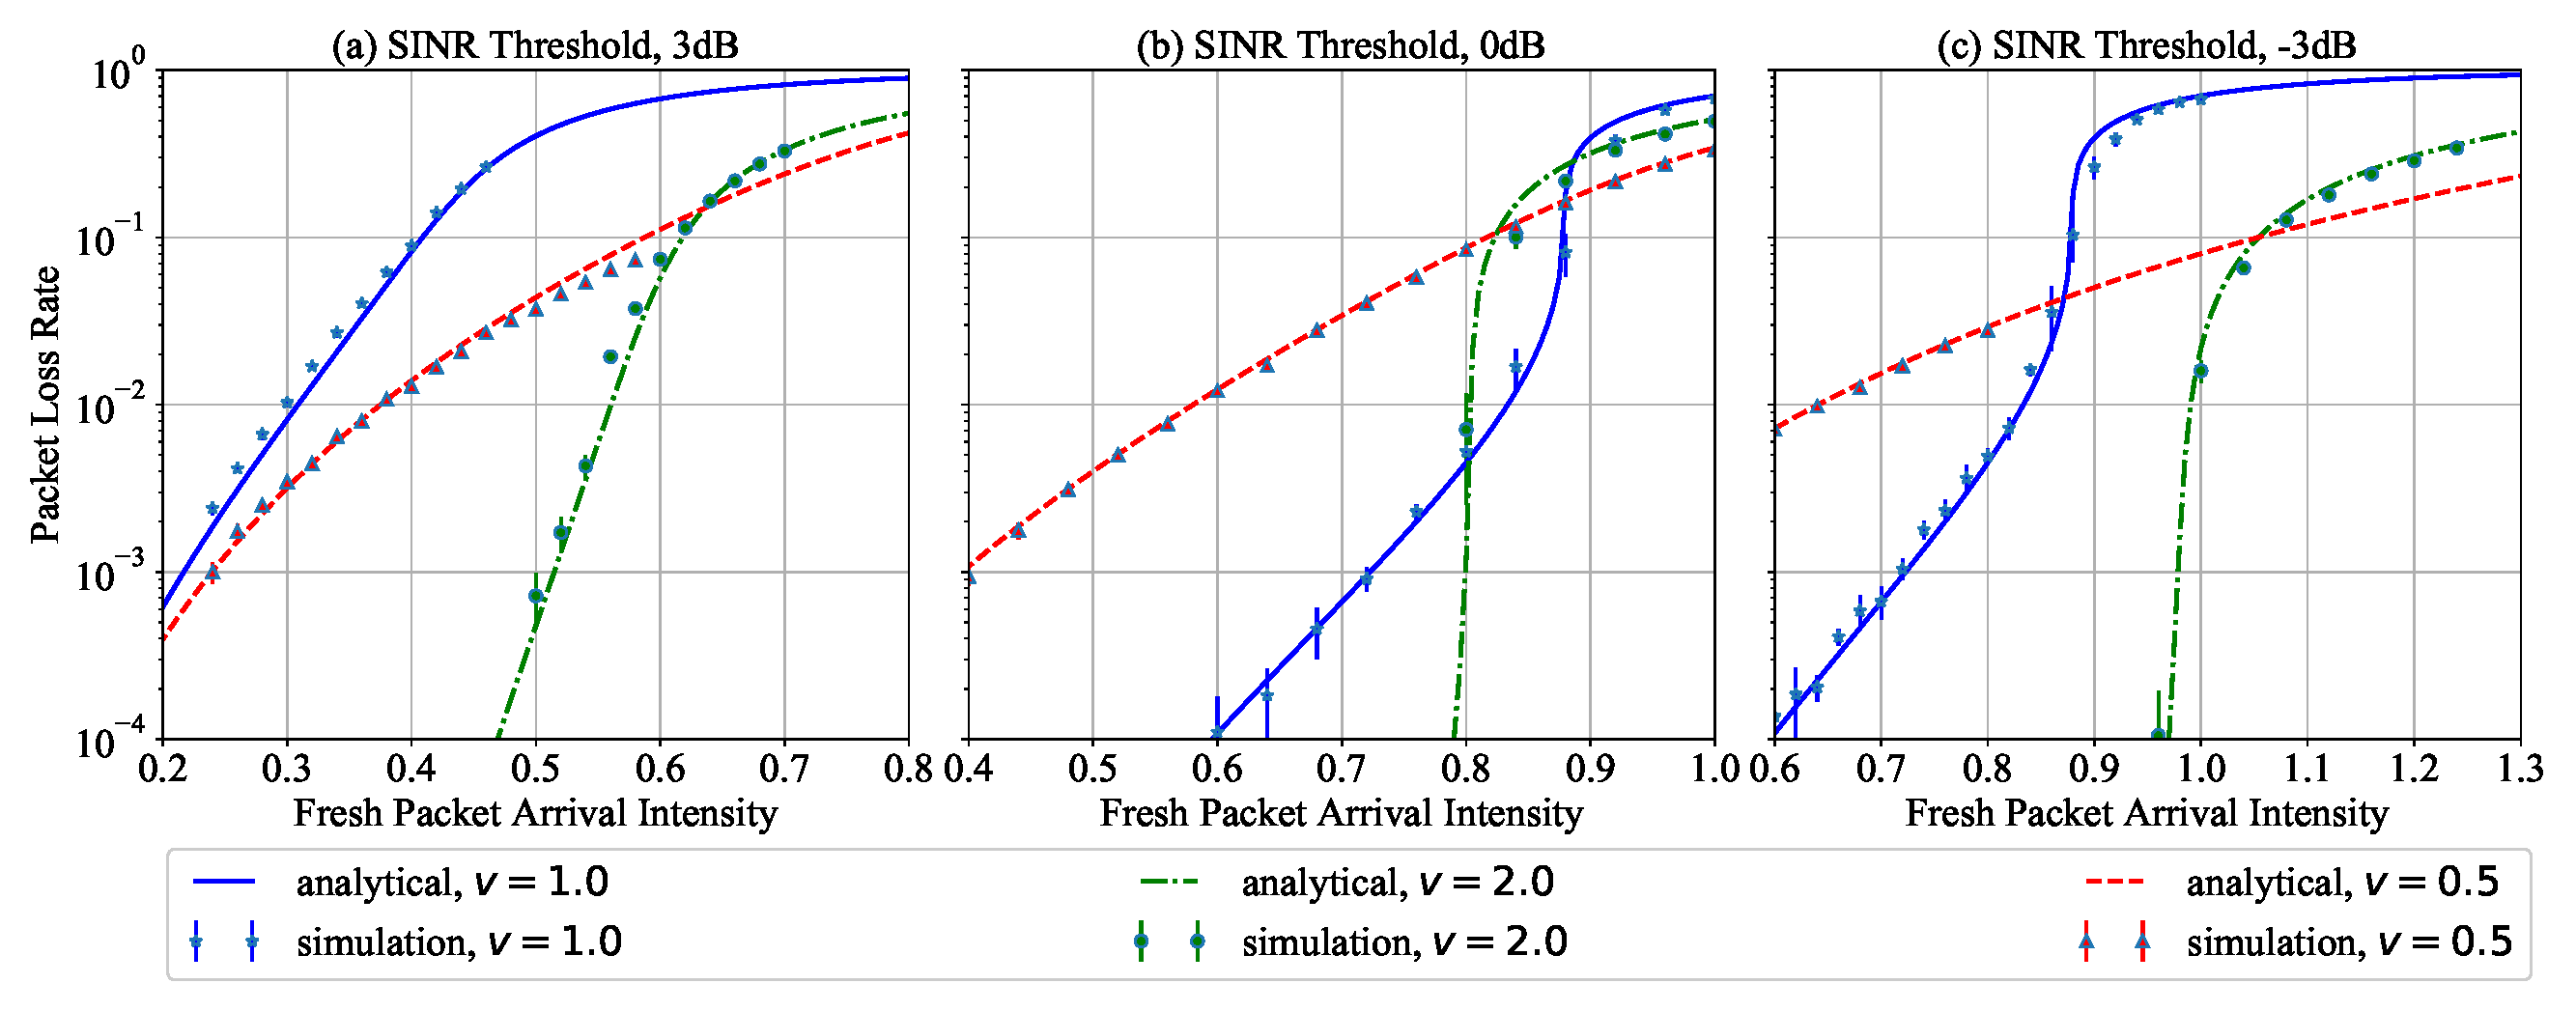
\includegraphics[width=1.0\linewidth]{Chapter4/Figures/packet_loss_rate_ci_with_ideal.eps}
	\caption{Packet loss rate of S-ALOHA under one ideal system}
	\label{fig:ideal_ci}
\end{figure}

\begin{figure}[!ht]
	\centering
	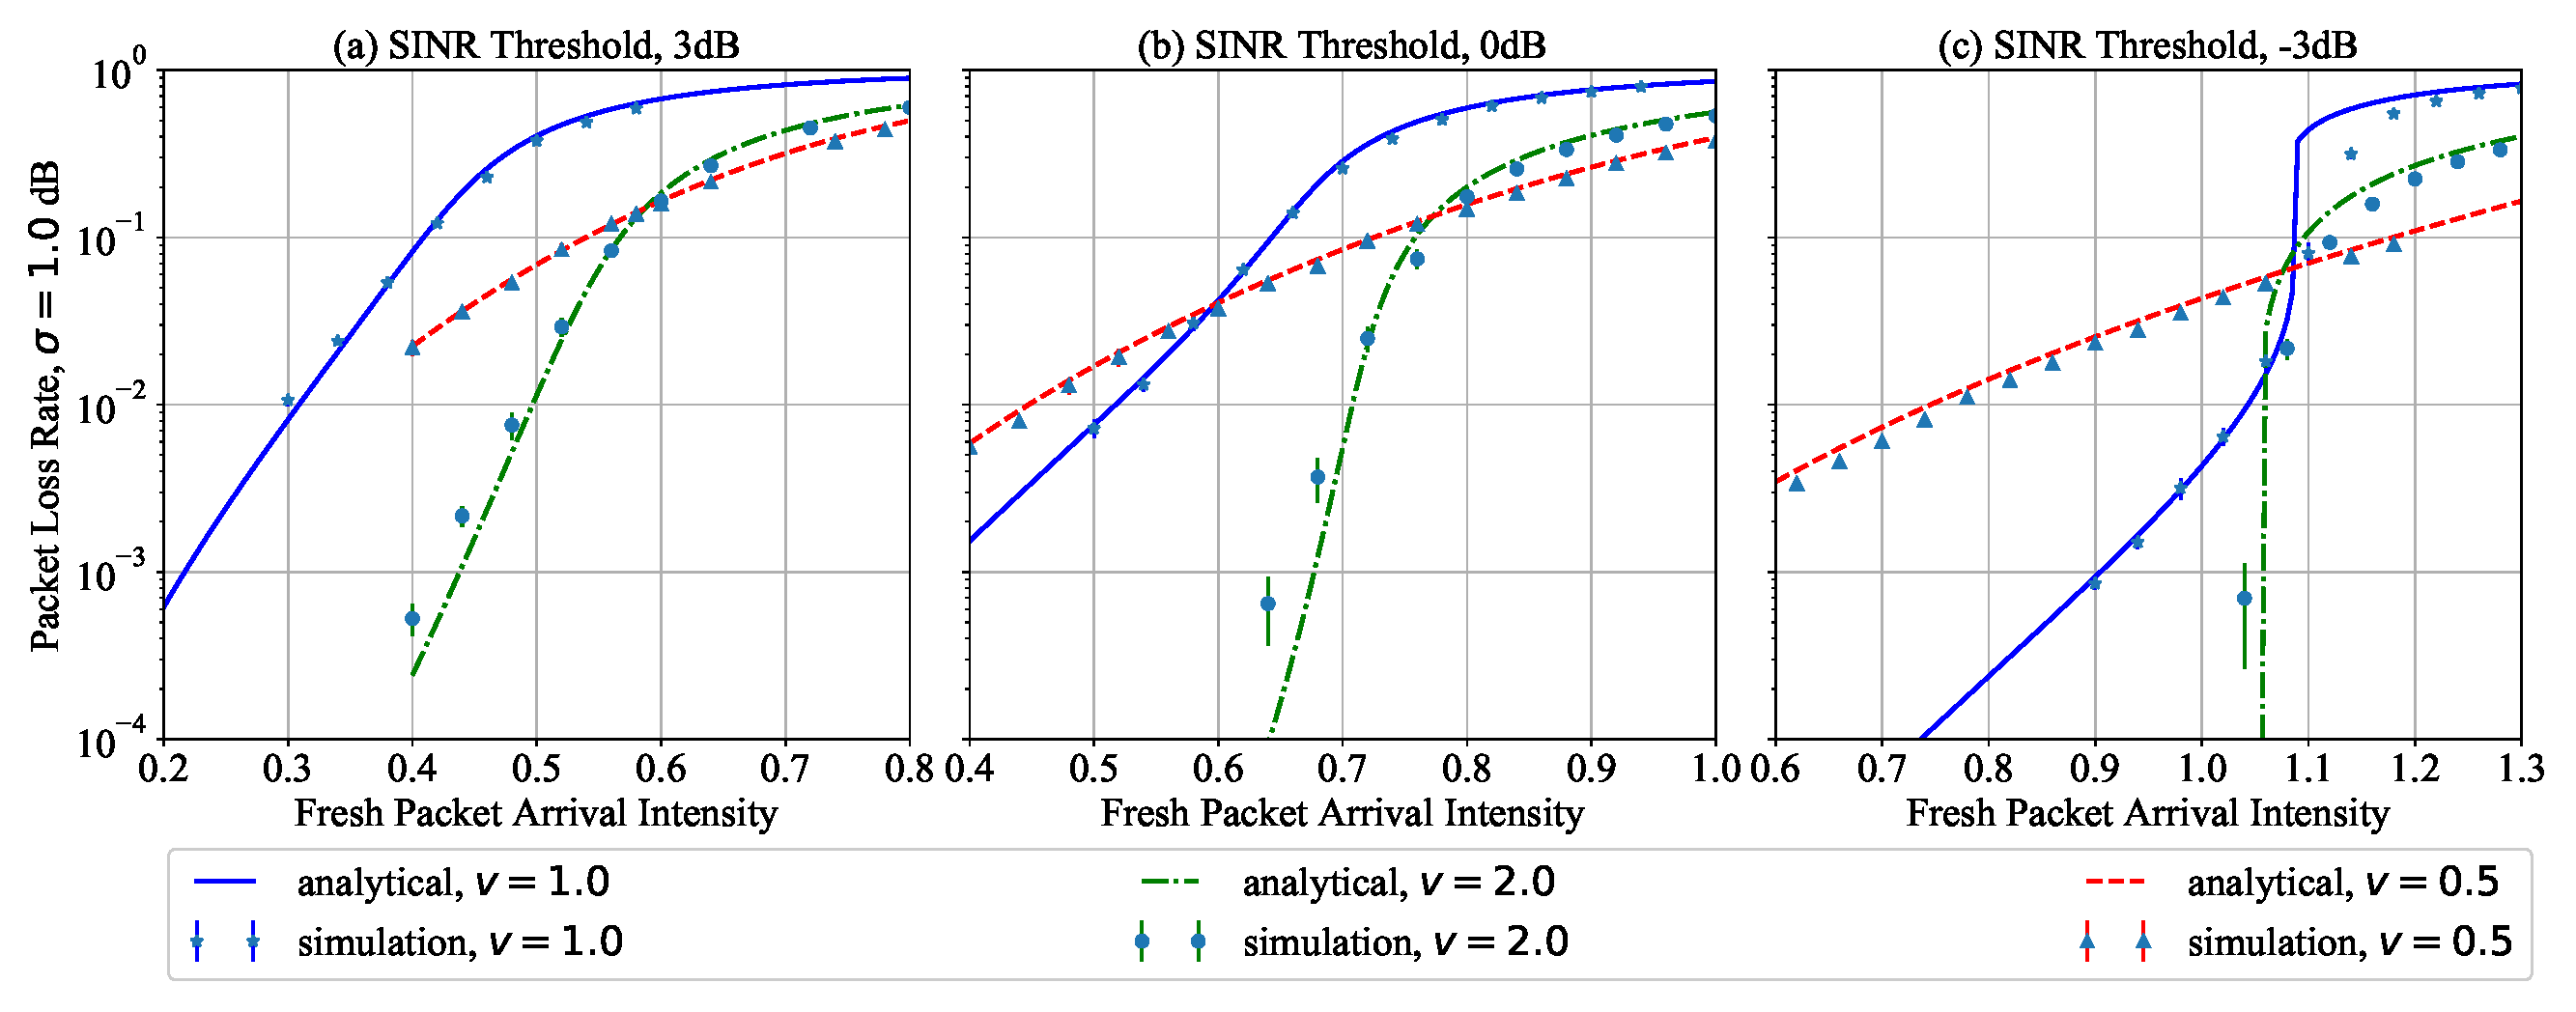
\includegraphics[width=1.0\linewidth]{Chapter4/Figures/packet_loss_rate_ci.eps}
	\caption{Packet loss rate of S-ALOHA under a wide-band system}
	\label{fig:ci}
\end{figure}

\begin{figure}[!ht]
	\centering
	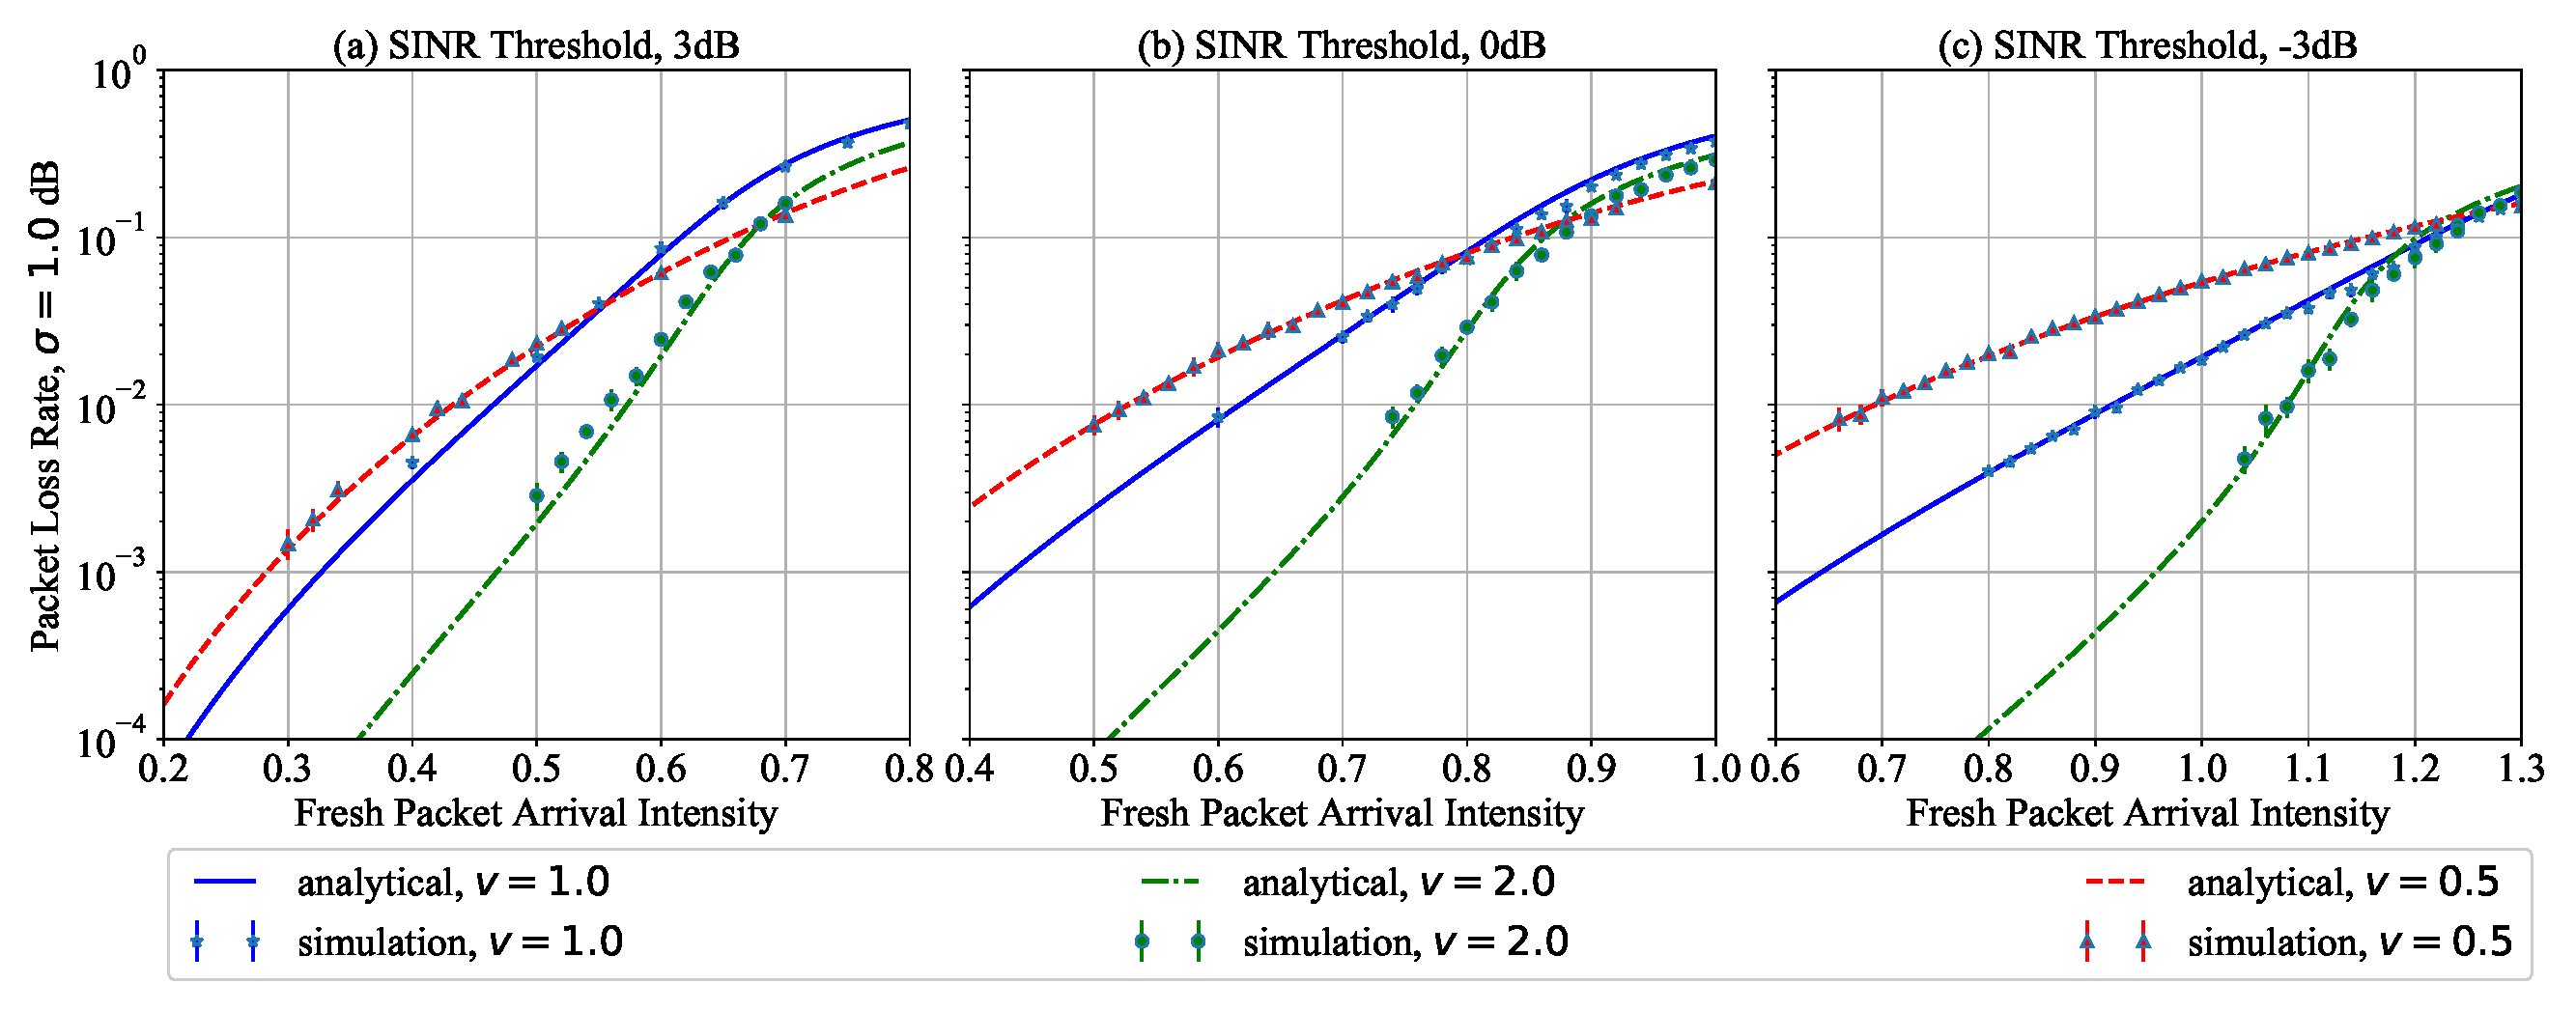
\includegraphics[width=1.0\linewidth]{Chapter4/Figures/packet_loss_rate_ci_with_fading_shadowing.eps}
	\caption{Packet loss rate of S-ALOHA in networks suffered fading and imperfect power control}
	\label{fig:ci_fading_shadowing}
\end{figure}

For a given arrival rate $\lambda T$, with our proposed analytical models, the probability vector can be obtained by less than $30$ iterations, within several seconds. This means that the proposed models can be integrated into M2M network dimensioning tools box.
\subsection{Performance evaluation under different settings}


\subsection{Evaluation for systems with imperfect power control}
The performance of S-ALOHA based M2M networks is evaluated in terms of packet loss rate, throughput, energy efficiency. Due to limitation of space, the performance of average number of transmission is not plotted in the figures. About the capture effect, SINR thresholds of $3$ dB, $0$ dB, $-3$ dB are considered. The case of perfect power control serves as comparison reference.
\begin{figure}[]
	\centering
	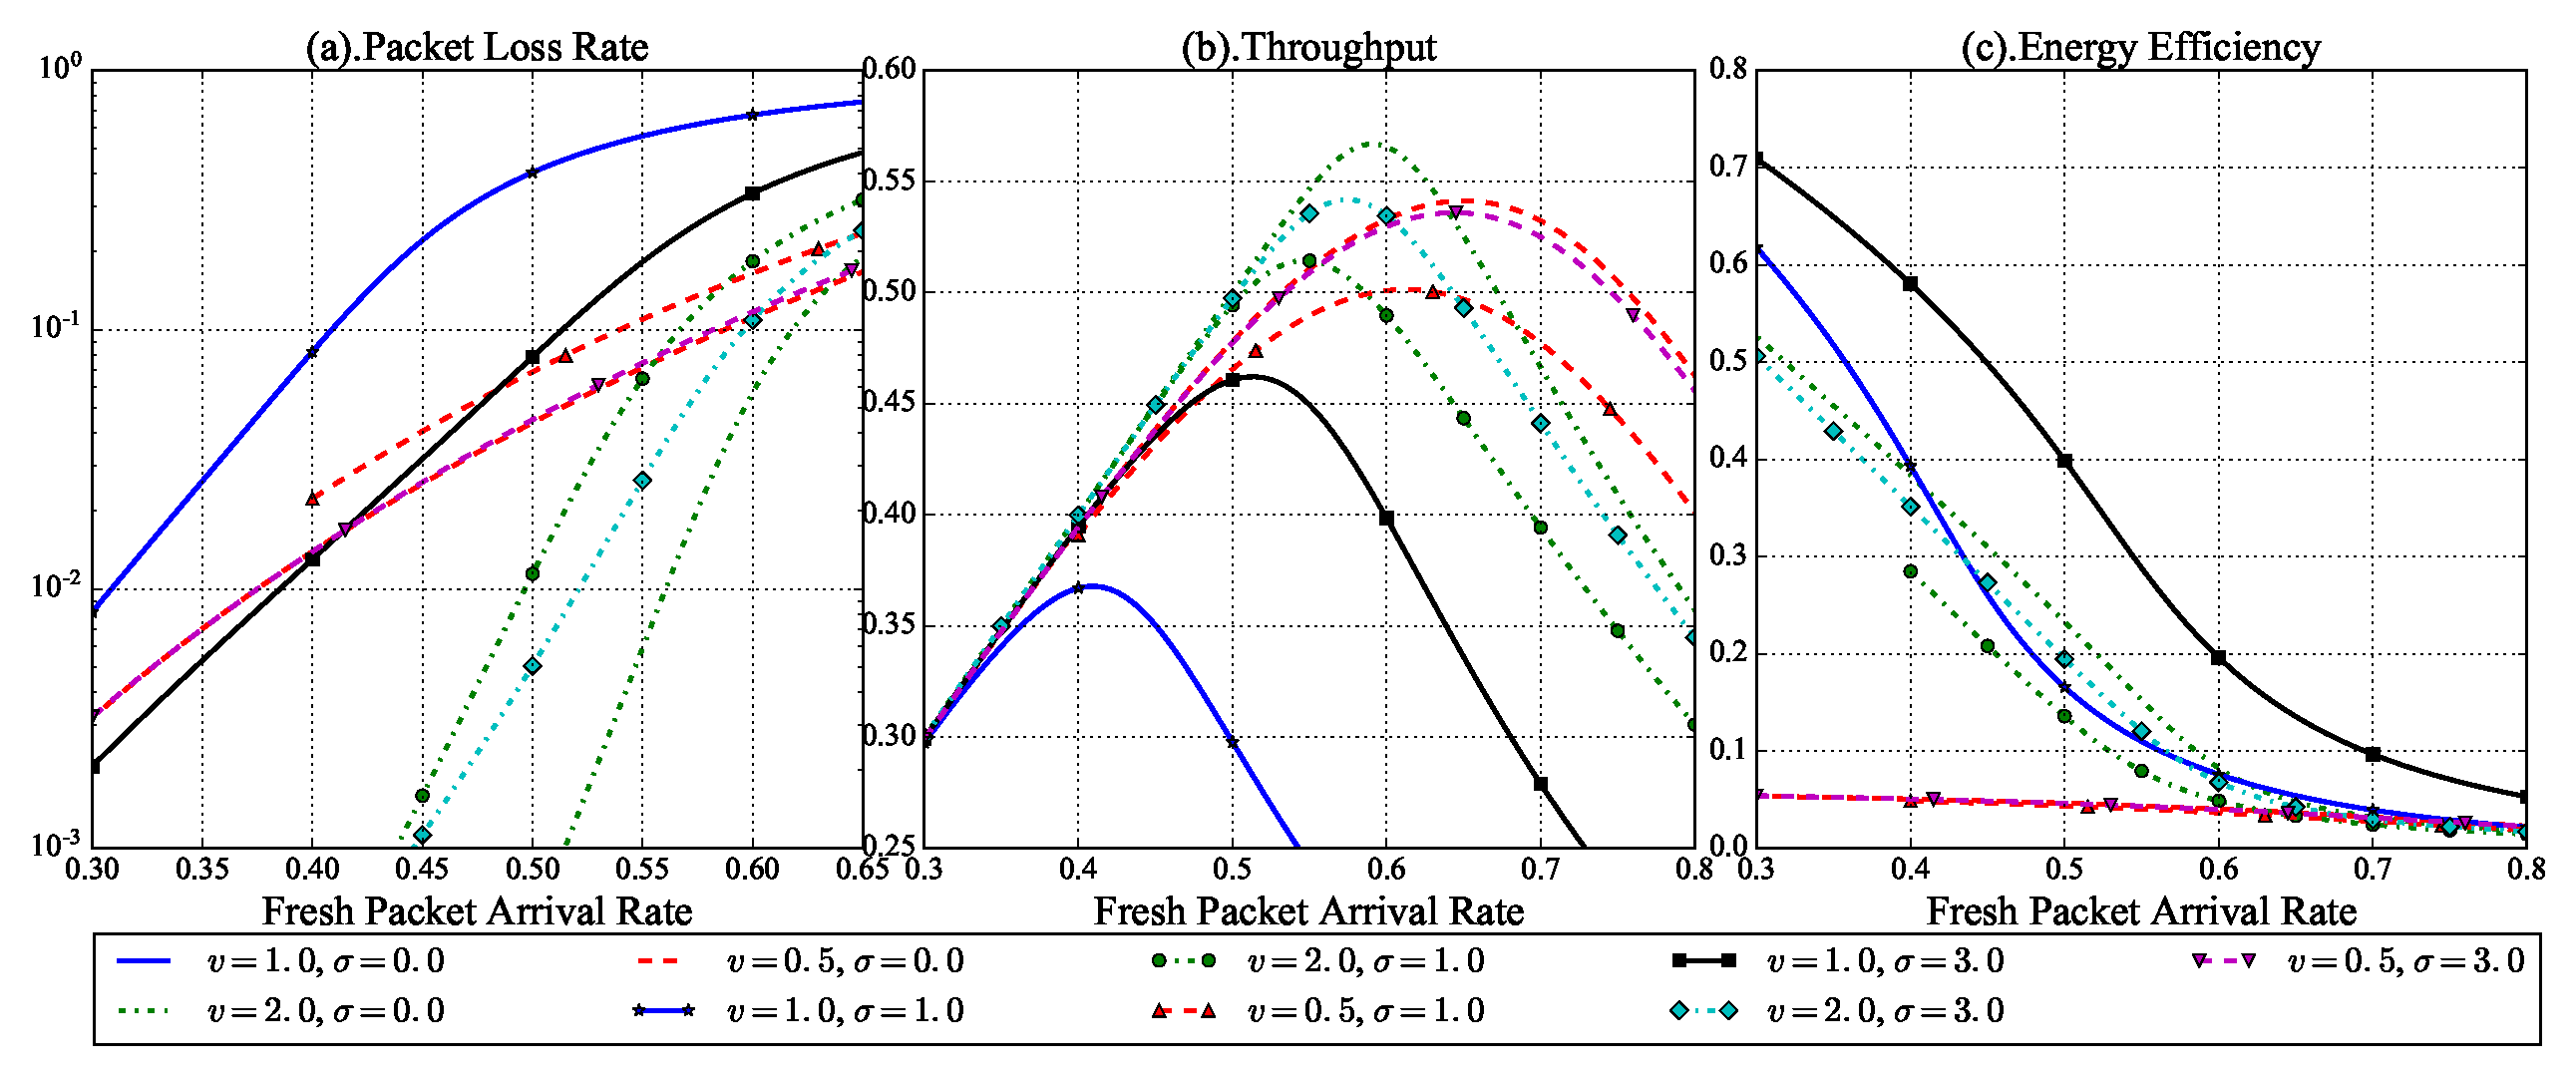
\includegraphics[width=1.0\linewidth]{Chapter4/Figures/shadowing_performance_case_3.0.eps}
	\caption{Performance comparison under SINR threshold $3$dB. Each sub-figure shows the comparison under three different power control error standard deviation $\sigma = 0, 1, 3$dB. Note that $\sigma=0.0$dB refers to the perfect power control case.}
	\label{fig:shadowing_performance}
\end{figure}

Fig.~\ref{fig:shadowing_performance} shows the performance with SINR threshold $3$dB. Each sub-figure of Fig.~\ref{fig:shadowing_performance} shows the comparison under three different power control error standard deviations $\sigma = 0, 1, 3$ dB. Note that $\sigma = 0.0$ dB refers to the perfect power control case. Some remarks obtained from Fig.~\ref{fig:shadowing_performance} are listed as follows:
\begin{itemize}[leftmargin=*, noitemsep]
	\item We observe that within a network applying identical transmit power strategy (the power incrementation factor $v=1$), when power control error standard variance is $1$dB, the performance of S-ALOHA is identical with perfect power control case (note that the curve of $v=1.0, \sigma=0.0$ and $v=1.0, \sigma=1.0$ are completely superposed). When the standard deviation of power control error is $3$dB, the S-ALOHA performance gets improved (comparing the solid line with square and solid line with stars). 
	Hence, applying identical transmit power strategy, the performance of all metrics get improved, with the degradation of power control precision ($\sigma$ varies from $0$ dB to $3$ dB). The reason is that power control error serves as a way to make transmit power levels more diverse and the presence of capture effect leverages such a received power level diversity.
	\item For other two strategies $v=2$ and $v=0.5$, the imperfect power control degrades the performance of S-ALOHA, because power control error reduces the transmit powers levels diversity introduced by factor $v$. 
	\item The comparison between different transmit power levels strategies with the same power control precision indicates that incremental or decremental strategies outperform the identical strategy except in term of energy efficiency. For example, in Fig.~\ref{fig:shadowing_performance}(c), S-ALOHA using identical transmit power outperforms than other strategies in terms of energy-efficiency. The reason is that these two strategies gain a high level transmit power diversity at the cost of more energy consumption. The energy-efficiency of decremental power strategy is always at low level, since this strategy requires to start with high power levels then decreases for the future retransmission.  
\end{itemize}

%The aforementioned observations tell us that: with presence of capture effect relatively high, instead of pursuing precise power control in device side, S-ALOHA can get improved with poor power control, since the latter make the transmit power levels more diverse.
Fig.~\ref{fig:shadowing_performance_0} shows the comparison result under capture ratio $0$dB. Compared with Fig.~\ref{fig:shadowing_performance}, the remarks that we get are as follows:
\begin{itemize}[leftmargin=*, noitemsep]
	\item Within a network in which devices are equipped with high level sensitivity receiver (i.e. capture ratio is $0$ dB), if the packet loss rate threshold is $10\%$, the system capacity is much higher (refer to Fig.~\ref{fig:shadowing_performance_0}(a)) than that in a network shown in Fig.~\ref{fig:shadowing_performance}(a).
	\item In this case, power control error brings a negative impact to the performance of S-ALOHA, no matter which transmit power strategy is employed. That means that if a MTC device is equipped with high level sensitivity receiver, the obtained system capacity gain in terms of arrival packet intensity is 
	partially neutralized cause of power control precision.
	\item Actually the perfect power control is just a theoretical situation. When power control error is inevitable, for all three power strategies, the performance of power control error $3$ dB is better than that of $1$ dB. The reason is that serious power control error makes the transmit power more diverse. 
	\item With such a capture ratio, the best choice of diversity strategy depends on the privileged performance metric. For example, for a M2M network preferring energy-efficiency to throughout, S-ALOHA with identical power strategy is recommended option. Otherwise, S-ALOHA with incremental power strategy is better. 
\end{itemize}
\begin{figure}[!th]
	\centering
	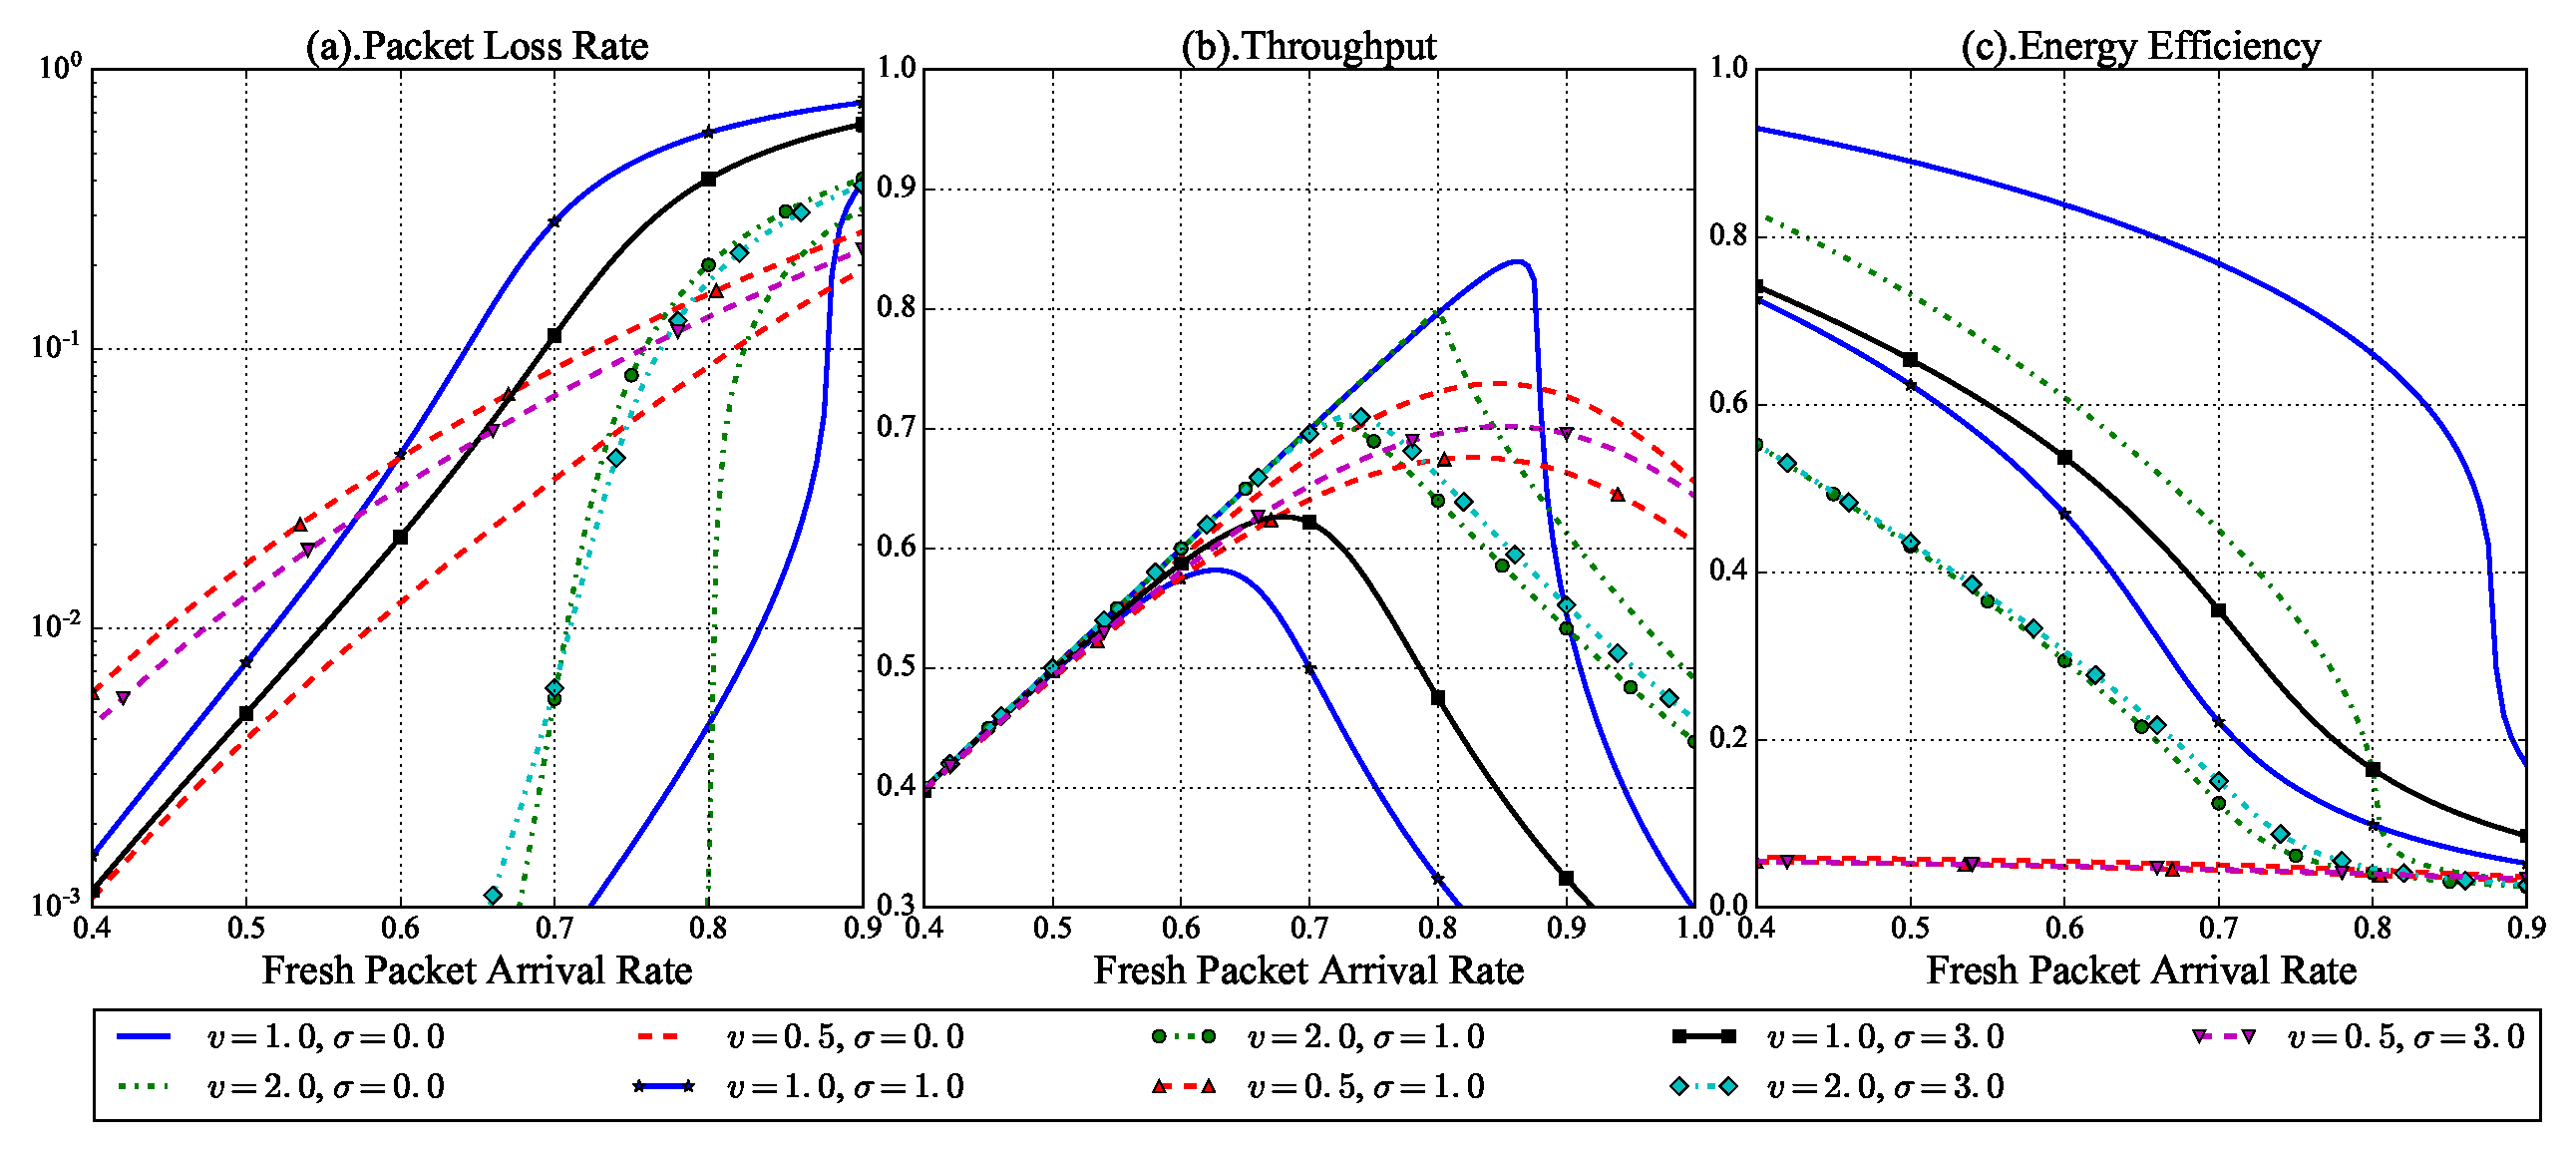
\includegraphics[width=1.0\linewidth]{Chapter4/Figures/shadowing_performance_case_0.0.eps}
	\caption{Performance comparison under SINR threshold $0$dB. Each sub-figure shows the comparison under three different power control error standard deviation $\sigma = 0, 1, 3$dB}
	\label{fig:shadowing_performance_0}
\end{figure}

Now we consider a M2M network with spectrum-spreading techniques. Thus, the capture ratio is negative (in unit of dB). Fig.~\ref{fig:shadowing_performance_-3} illustrates the S-ALOHA performance with $-3$ dB as SINR threshold. The observations and remarks obtained are:
\begin{itemize}[leftmargin=*, noitemsep]
	\item As the decrease of capture ratio, the system capacity in terms of arrival packet intensity is increased, compared with Fig.~\ref{fig:shadowing_performance_0}.
	\item With spectrum spreading technique, no matter which transmit power strategy is applied, the power control error always has a positive impact on S-ALOHA. 
	\item S-ALOHA achieves a better performance when the power control is more precise (For example, compare the solid line with star markers and that with square marker in Fig.~\ref{fig:shadowing_performance_-3}(a)). That means that in a S-ALOHA M2M network with spectrum-spreading techniques, S-ALOHA performance is better when all MTC devices equi
	\item In addition, the choice of transmit power diversity depends on fresh packet arrival rate. For example, when the standard deviation of power control error is $1$dB, if networks based on S-ALOHA are still unsaturated (i.e, with fresh arrival rate less than $1.1$), identical strategy is better than others. With arrival rate greater than $1.1$, the throughput  is sharply reduced. The decremental strategy starts to be a better choice.
\end{itemize}

\begin{figure}[!th]
	\centering
	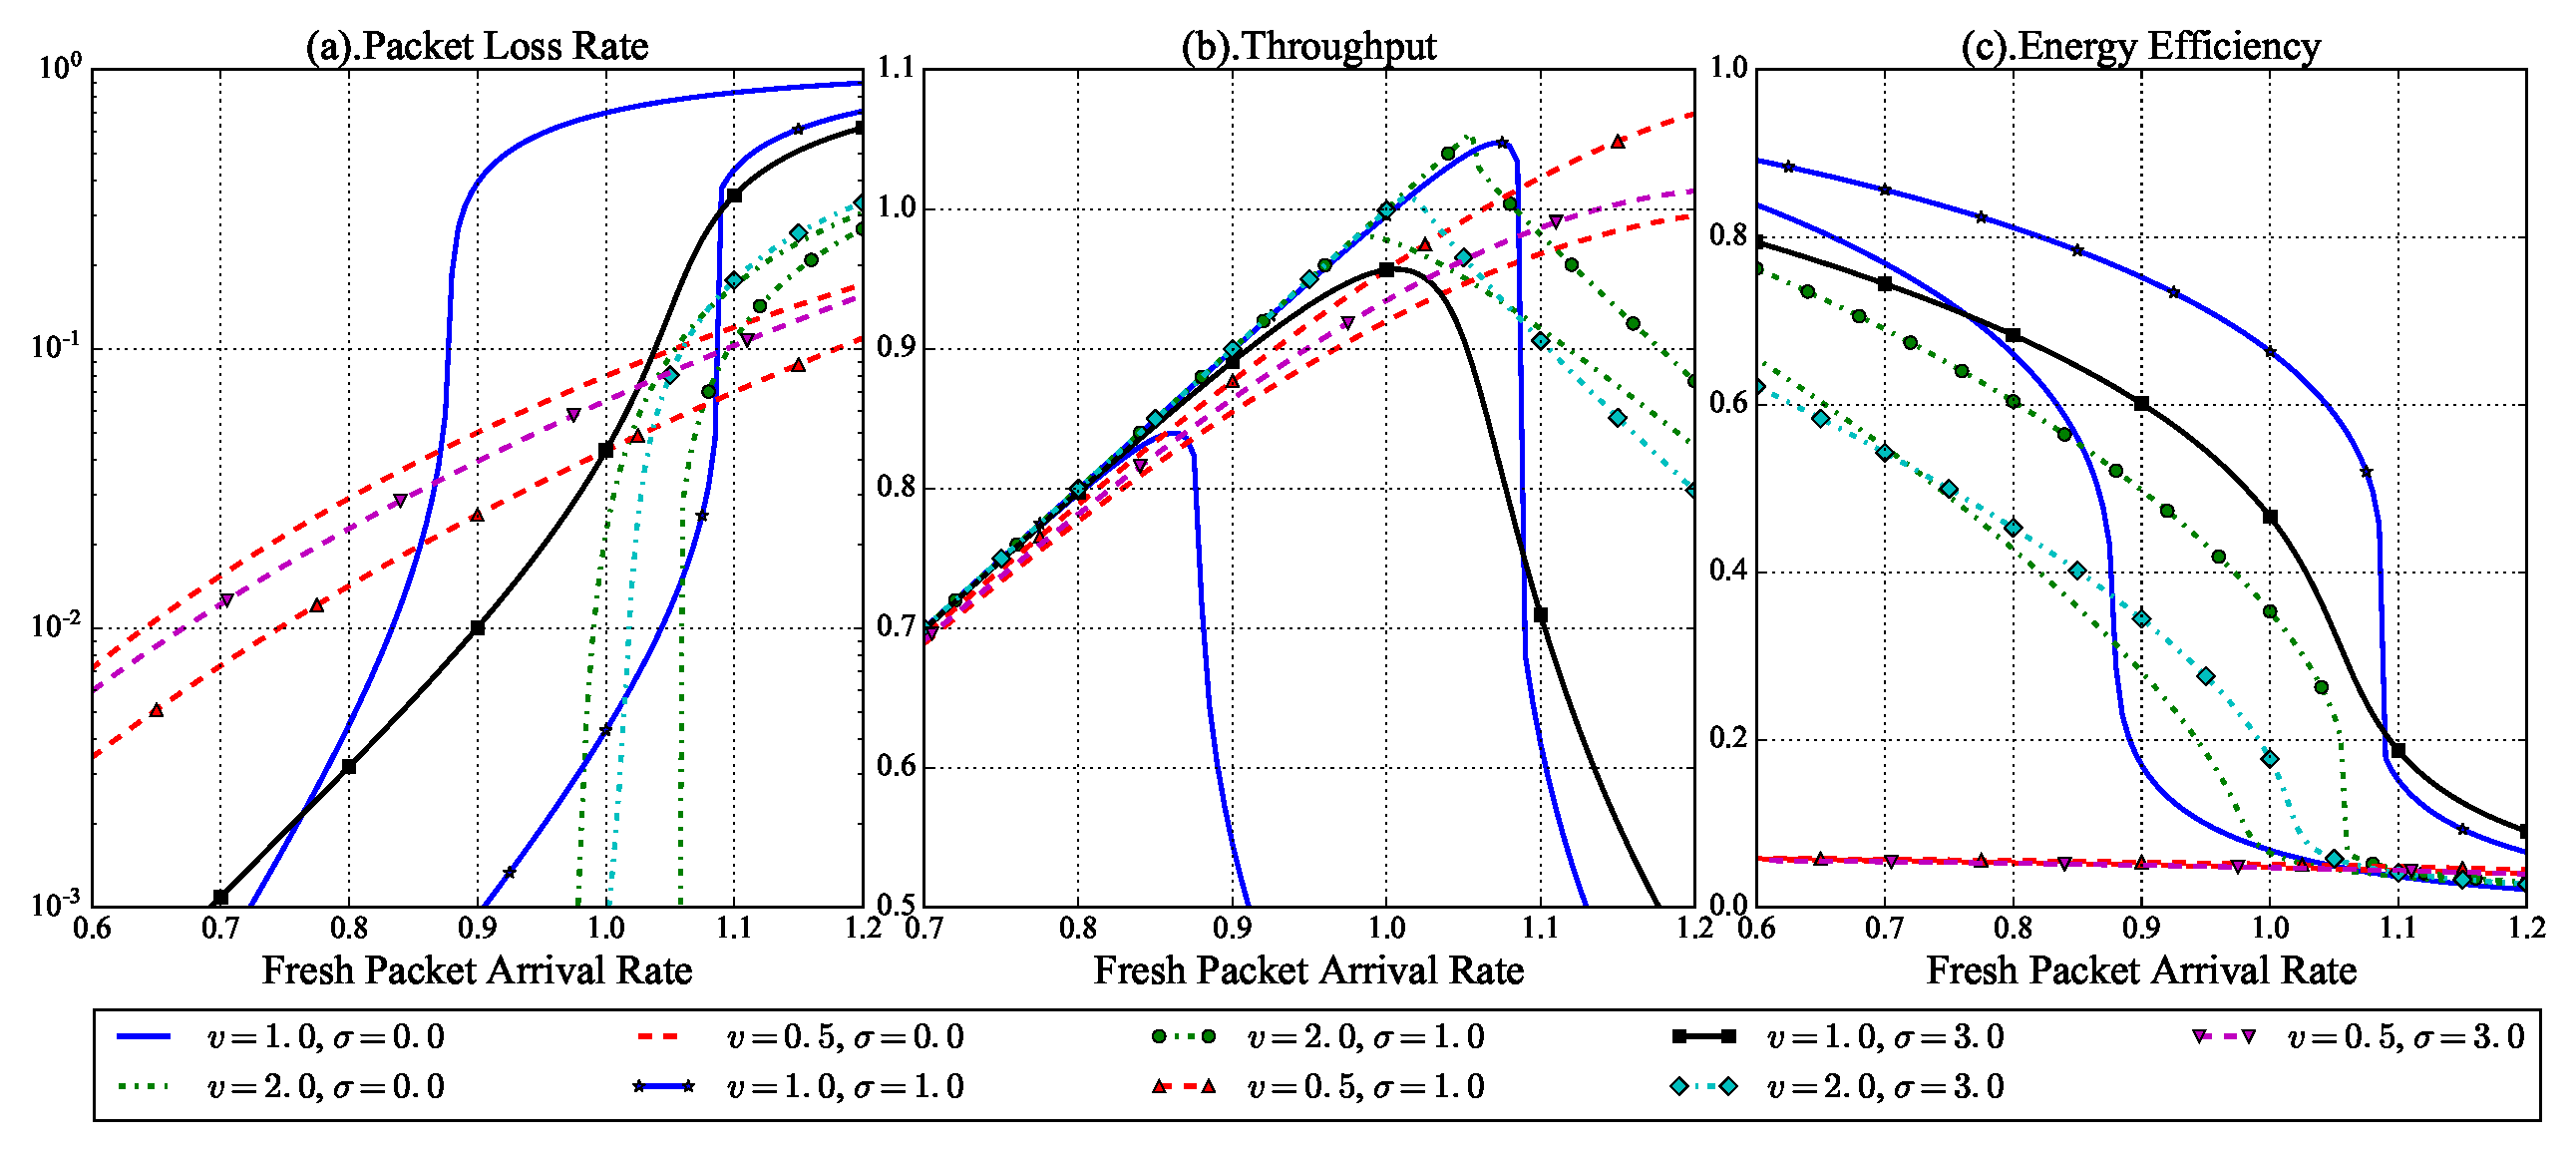
\includegraphics[width=1.0\linewidth]{Chapter4/Figures/shadowing_performance_case_-3.0.eps}
	\caption{Performance comparison under SINR threshold $-3$dB. Each sub-figure shows the comparison under three different power control error standard deviation $\sigma = 0, 1, 3$dB}
	\label{fig:shadowing_performance_-3}
\end{figure}


\subsection{Evaluation for systems suffering fading and imperfect power control}
We still choose the ideal system model as comparison reference. The narrow band system for example LoRaWAN. still use power control.
Since narrow band system has no spectrum spreading techniques, we just consider capture ratio $3$ dB and $0$dB.

Fig.~\ref{fig:fading_shadowing_performance_3} and Fig.~\ref{fig:fading_shadowing_performance_0} respectively show the S-ALOHA performance when capture ratio is $3$ dB, $0$ dB. The remarks that we derive from both figures are as follows:
\begin{itemize}[leftmargin=*, noitemsep]
	\item For identical and decremental transmit power strategies, the fading effect improves the S-ALOHA performance. 
	\item For incremental strategy, we note that in terms of packet loss rate, there exists one critical point (about $0.55$ in Fig.~\ref{fig:fading_shadowing_performance_3}(a) and $0.68$ in Fig.~\ref{fig:fading_shadowing_performance_0}(a)). That means that the packet loss rate of S-ALOHA in a network suffering fading and imperfect power control get improved only if the fresh arrival packet intensity is greater than a certain critical point. For other metrics, such as throughput, energy efficiency, the performance get improved without a critical point.
\end{itemize}

\begin{figure}[!th]
	\centering
	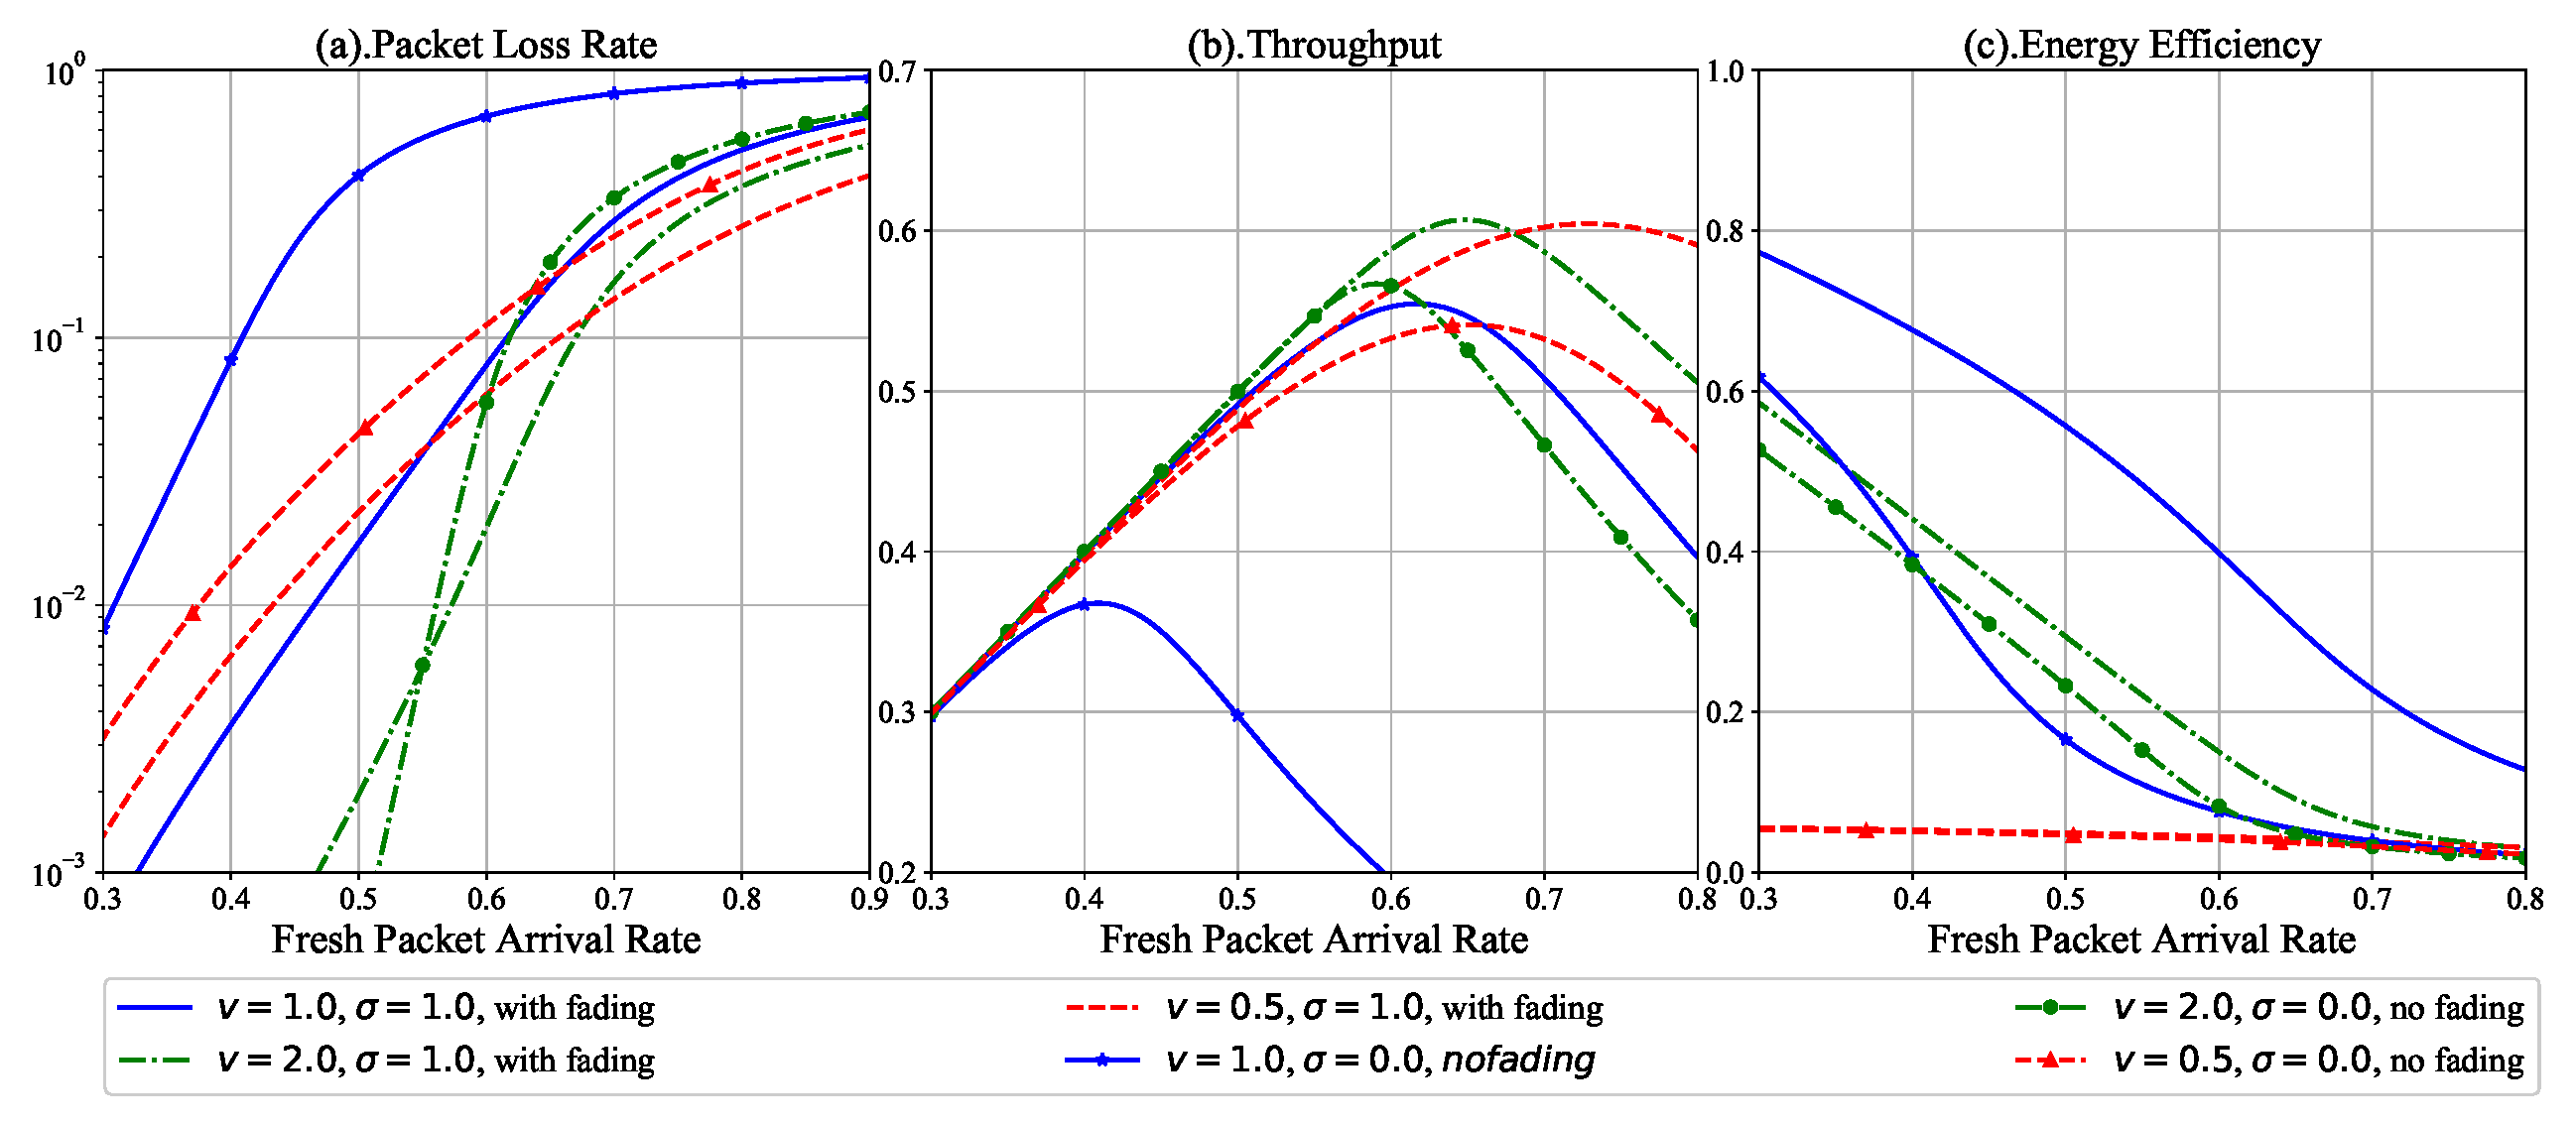
\includegraphics[width=1.0\linewidth]{Chapter4/Figures/fading_shadowing_performance_case_3.0.eps}
	\caption{Performance comparison under SINR threshold $3$dB. Each sub-figure shows the comparison under three different power control error standard deviation $\sigma = 1$dB.}
	\label{fig:fading_shadowing_performance_3}
\end{figure}

\begin{figure}[!th]
	\centering
	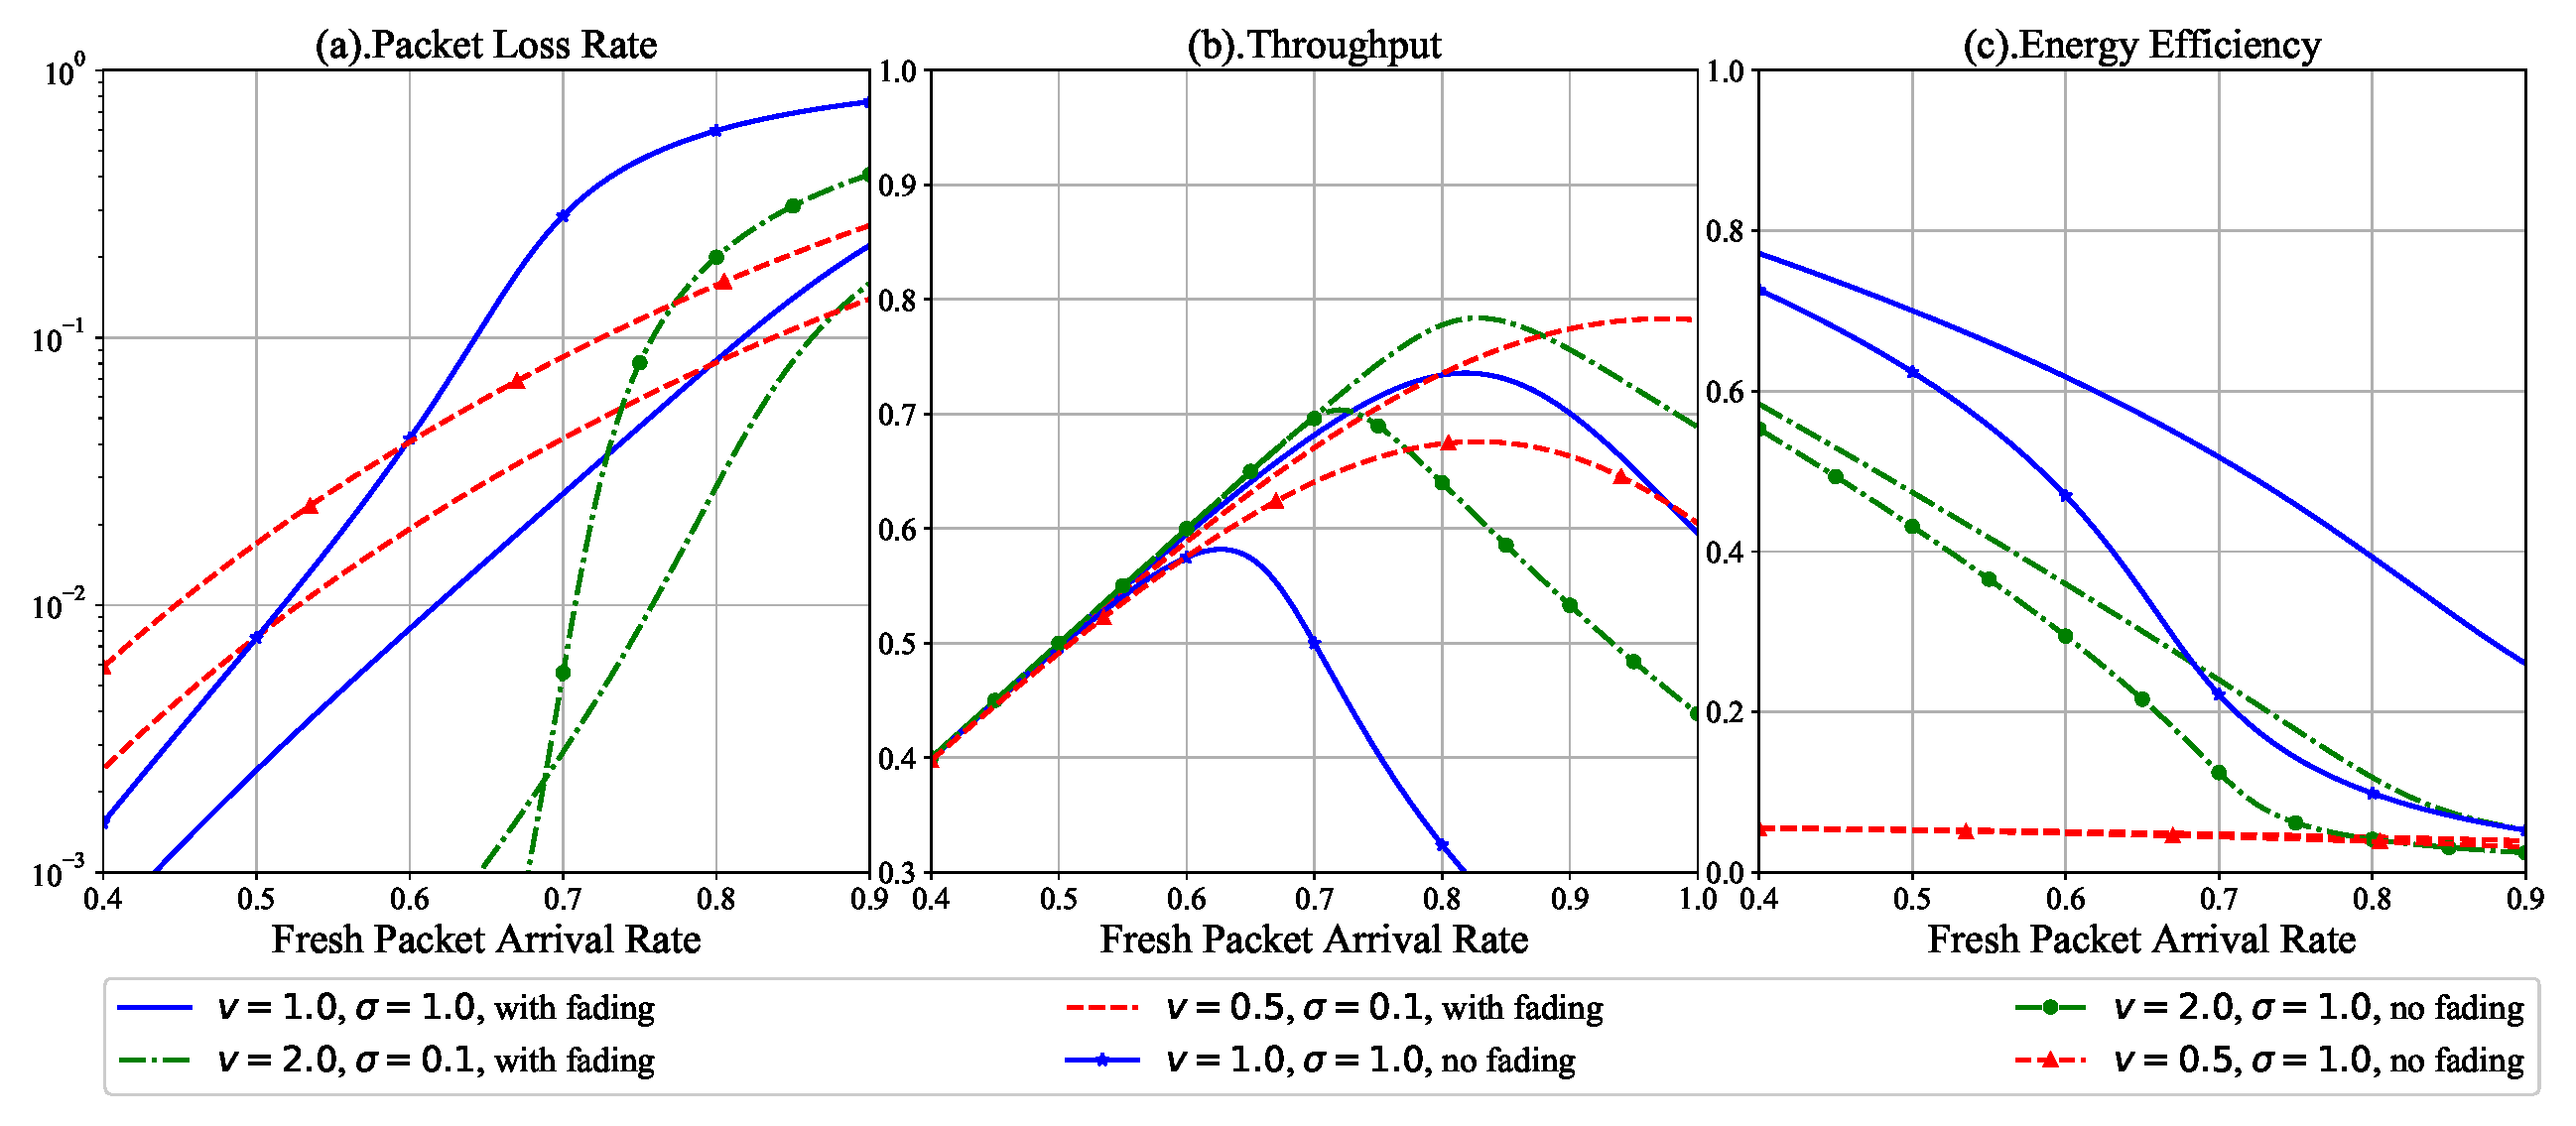
\includegraphics[width=1.0\linewidth]{Chapter4/Figures/fading_shadowing_performance_case_0.0.eps}
	\caption{Performance comparison under SINR threshold $0$dB. Each sub-figure shows the comparison under three different power control error standard deviation $\sigma =1$dB.}
	\label{fig:fading_shadowing_performance_0}
\end{figure}

%\begin{figure}[!th]
%	\centering
%	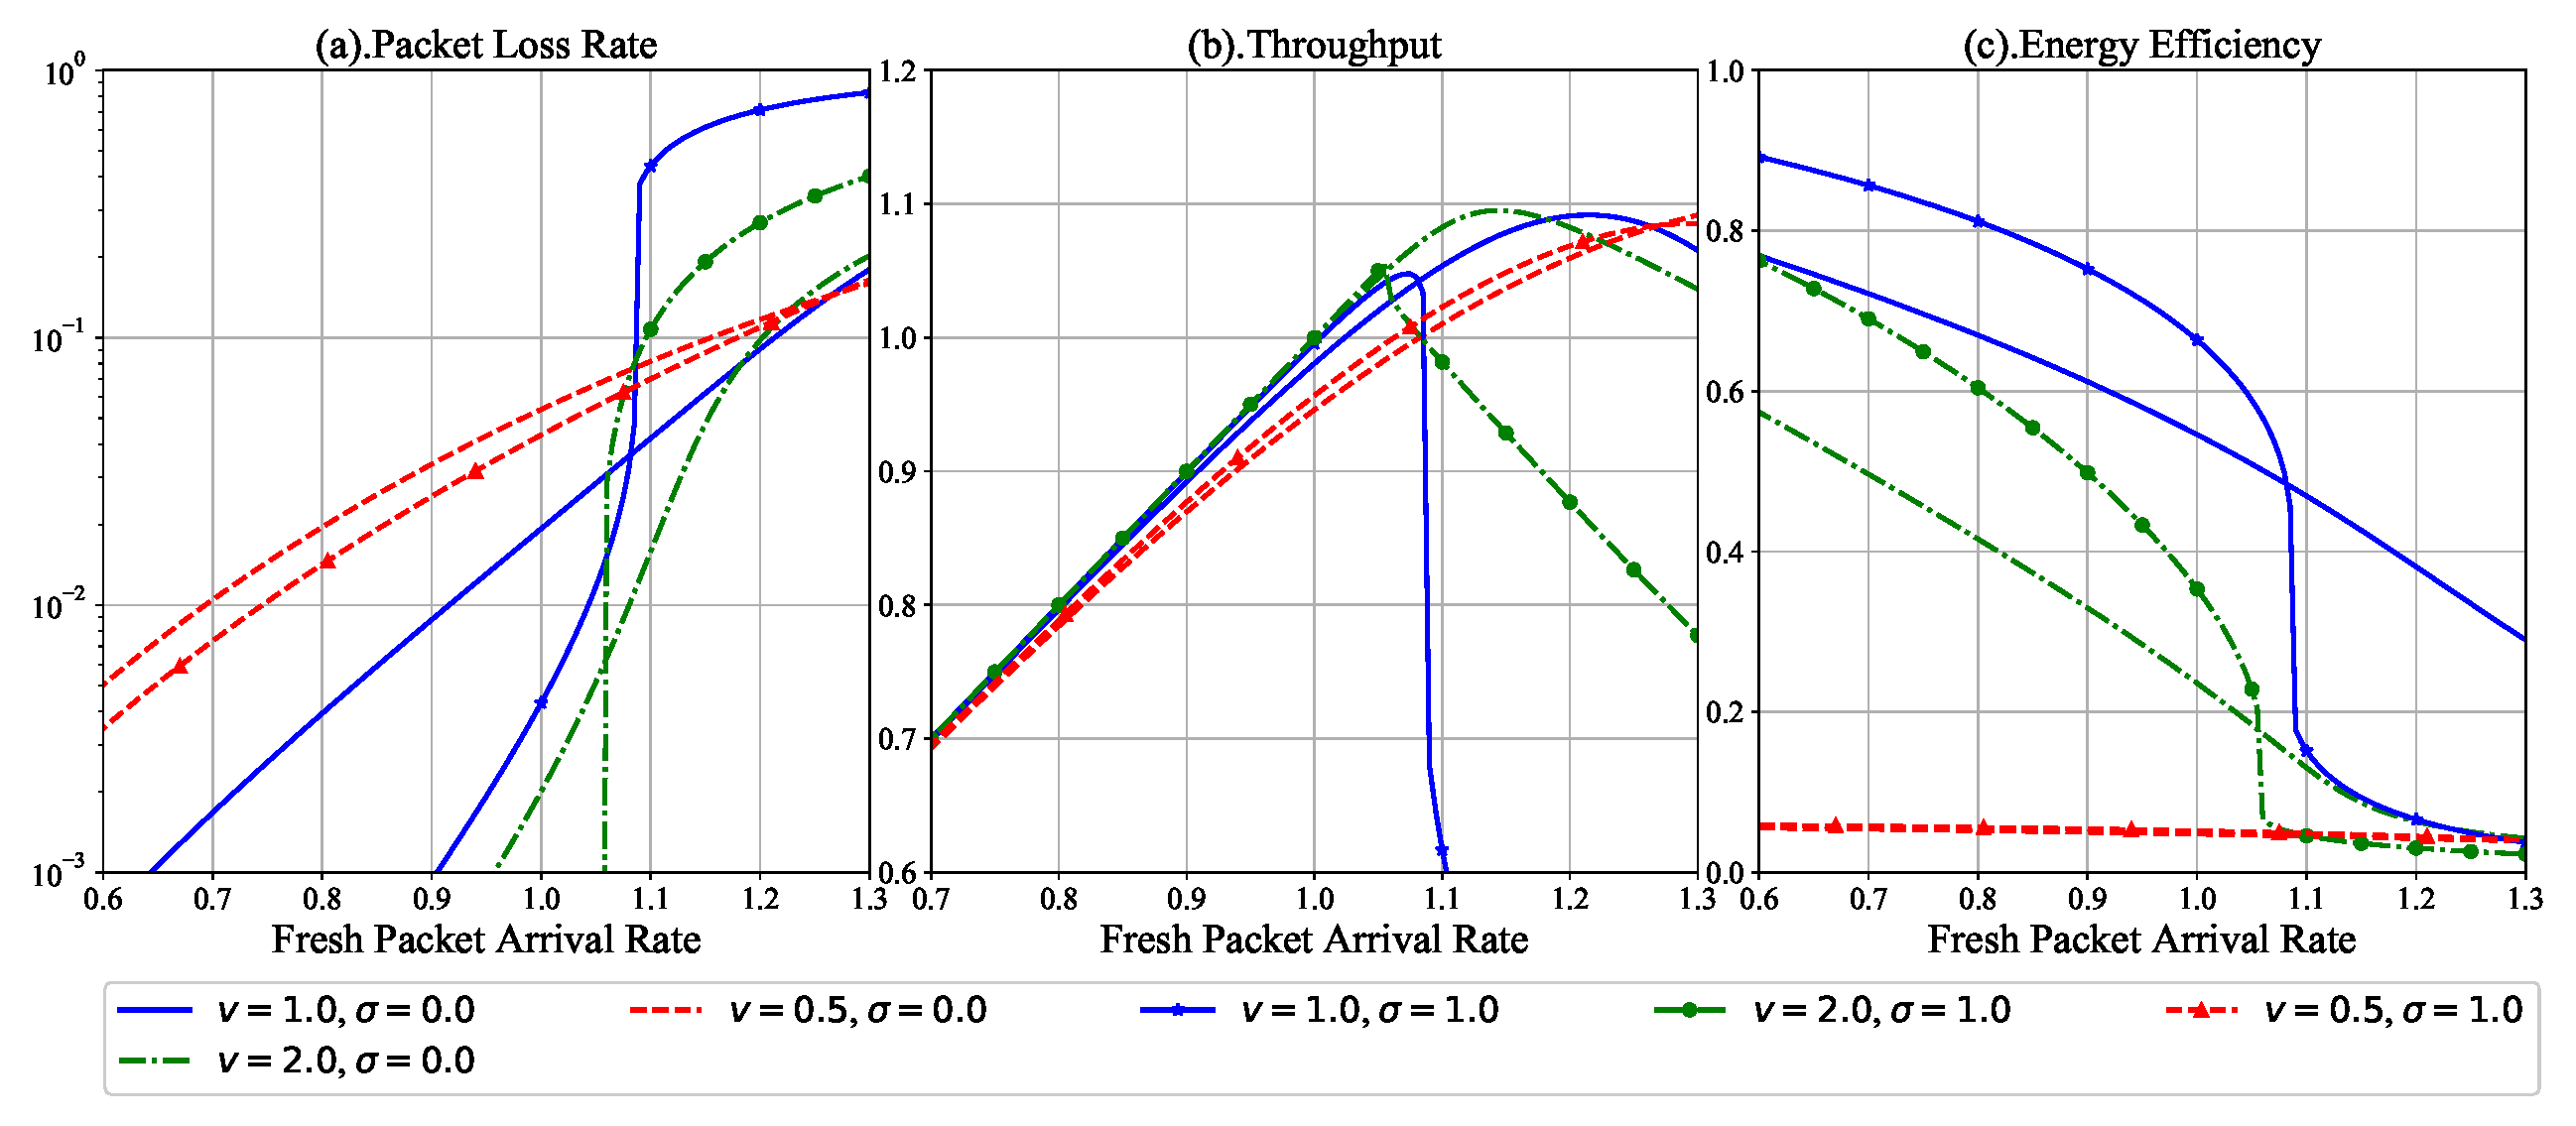
\includegraphics[width=1.0\linewidth]{Chapter4/Figures/fading_shadowing_performance_case_-3.0.eps}
%	\caption{Performance comparison under SINR threshold $-3$dB. Each sub-figure shows the comparison under three different power control error standard deviation $\sigma =1$dB.}
%	\label{fig:fading_shadowing_performance_-3}
%\end{figure}
% 
%Precisely, it has an obvious impact when power increment factor is less than its standard error.


%\begin{figure}[!th]
%	\centering
%	\includegraphics[width=1.0\linewidth]{Figures/logarithme_shadowing_case1.eps}
%	\caption{The Packet Loss Rate evolution with respect to the fresh packet arrival intensity. The SINR threshold for a successful packet transmission is $3$ dB. The effects of power increment, power decrement and no power change are all shown in the same figure.}
%	\label{fig:shadowing_case1}
%\end{figure}
%
%\begin{figure}[!th]
%	\centering
%	\includegraphics[width=1.0\linewidth]{Figures/logarithme_shadowing_case2.eps}
%	\caption{The Packet Loss Rate evolution with respect to the fresh packet arrival intensity. The SINR threshold for a successful packet transmission is $0$ dB. The effects of power increment, power decrement and no power change are all shown in the same figure.}
%	\label{fig:shadowing_case2}
%\end{figure}
%
%\begin{figure}[!th]
%	\centering
%	\includegraphics[width=1.0\linewidth]{Figures/logarithme_shadowing_case3.eps}
%	\caption{The Packet Loss Rate evolution with respect to the fresh packet arrival intensity. The SINR threshold for a successful packet transmission is $-3$ dB. The effects of power increment, power decrement and no power change are all shown in the same figure.}
%	\label{fig:shadowing_case3}
%\end{figure}


%\subsection{Fading and imperfect power control}
%\subsubsection{Case1: 3dB}
%From Fig.~\ref{fig:fading_case1}, we observe that when the predefined SINR threshold is set as $3$dB, for the case power increment, power decrement and no power change, the simulation and analytical results are well coherent. Also, we find that for the packet loss rate range of interest (i.e., from $10^{-2}$ to $10^{-1}$), it is the power increment case which always has the best performance (i.e., support higher packet arrival intensity with same packet loss loss rate)
%\begin{figure}[!th]
%	\centering
%	\includegraphics[width=\linewidth]{Figures/logarithme_fading_case1.eps}
%	\caption{The Packet Loss Rate evolution with respect to the fresh packet arrival intensity. The SINR threshold for a successful packet transmission is $3$ dB. The effects of power increment, power decrement and no power change are all shown in the same figure.}
%	\label{fig:fading_case1}
%\end{figure}
%
%\subsubsection{Case2: 0dB}
%From Fig.~\ref{fig:fading_case2}, we observe that the simulation result is well superposed with analytical result. Also, we find that for the packet loss rate range of interest (i.e., from $10^{-2}$ to $10^{-1}$), it is the power increment case which always has the best performance (i.e., support higher packet arrival intensity with same packet loss loss rate). However, around packet loss rate as $10^{-1}$, the performance gain of power increment case (dashdot line) is small compared with case of power decrement (dashed line).
%\begin{figure}
%	\centering
%	\includegraphics[width=\linewidth]{Figures/logarithme_fading_case2}
%	\caption{The Packet Loss Rate evolution with respect to the fresh packet arrival intensity. The SINR threshold for a successful packet transmission is $0$ dB.}
%	\label{fig:fading_case2}
%\end{figure}
%
%\subsubsection{Case3: -3dB}
%From Fig.~\ref{fig:fading_case3}, we observe that the simulation result is well superposed with analytical result. Also, we find that for the packet loss rate range of interest (i.e., from $10^{-2}$ to $10^{-1}$), it is the power increment case which always has the best performance (i.e., support higher packet arrival intensity with same packet loss loss rate). However, around packet loss rate as $10^{-1}$, the performance gain of power increment case (dashdot line) is small compared with case of identical power (continuous line).
%\begin{figure}
%	\centering
%	\includegraphics[width=\linewidth]{Figures/logarithme_fading_case3}
%	\caption{The Packet Loss Rate evolution with respect to the fresh packet arrival intensity. The SINR threshold for a successful packet transmission is $-3$ dB.}
%	\label{fig:fading_case3}
%\end{figure}

\section{Conclusion and Future works}
\label{sec:icc17-conclusion}
In this chapter, we have presented an accurate analytical model capable of estimating steady-state performances, i.e., packet loss rate, throughput, energy efficiency and average number of transmissions, of S-ALOHA based LPWAN networks. The model accounts for various performance-affecting factors, such as capture effect, diversity of transmit power levels, power control error, which have not been jointly considered in previous researches and can not be handled by widely used Bianchi's model.

We employ numerical integration method to calculate cumulative distribution function (CDF) of total interference from its corresponding characteristic function and fixed point analysis to solve the problem. The computational complexity is reduced by combining the recent research effort about log-normal sum (LNS) approximation problem and mathematical skills used in finance domain. The accuracy of the proposed model is confirmed by simulation. Due to its low complexity, our model can be used as a dimensioning tool to accurately and rapidly estimate the steady-state system outage capacity and throughput of  S-ALOHA-based LPWAN networks. With our proposed models, we also obtain some design guidelines for S-ALOHA.
%Note: Our proposed model also enables to study the case where the power increment factor is a random number.
%Our proposed model is also easy to be extended to multichannel case.
%
%In this paper, we develop a systematic framework to study the 
%
%For transmit power diversity strategies, we consider three strategies: blablabla... We also study the power control impact.
%The contributions of this paper are:
%\begin{inparaenum}[1)]
%	\item propose an iterative analytical framework taking into account capture effect, power control error and diversity of transmit power level, 
%	%	different from \qsong{We have not used the popular Markovian technique, i.e., Bianchi model, to analyze the steady state performance. We just use a fixed point analysis to get a steady state probability vector (detailed in system model part), which allows us to get some performance metrics such as packet loss rate, throughput, expected number of a packet delivered, etc. In my opinion, one limitation of Bianchi model and its derivaties is not able (or is very complicated if be able to do this) to process the case where transmission failure probability is different for each transmission. The advantage of our method is, we just concern how to use computer to get the target probability vector. Once we got this probability vector, other performance metrics can be easily calculated. Maybe be better to be done at last step...}largely used Markovian technique to analyze the steady state packet loss rate based on Poisson's split theorem. The analytical framework can be used to dimension the LPWAN networks with low computational complexity.
%	\item employ the recent research effort about log-normal distribution type variable approximation and mathematical skills largely used in finance domain to reduce the computational complexity;
%\end{inparaenum} 


In future work, we will add the performance evaluation for narrow-band systems where fading is considered. We will also take into account the impact of  interferences from multiple base stations in the proposed model.




